 %%%%%%%%%%%%%%%%%%
%%%   Template para utilização do plano de estágio %%%
%%%%%%%%%%%%%%%%%%

%% Preencher apenas os dados entre {}

\documentclass[12pt,openright,oneside,a4paper,english,french,spanish,brazil]{unifil}

\titulo{Sistema de Rotas Inteligentes}
\autor{Danilo Iglesia Da Silva} % Nome do aluno
\instituicao{Centro Universitário Filadélfia}
\local{Londrina}
\data{2026} % Ano de publicação
\preambulo{Curso de bacharelado em Ciência da Computação} % Nome do curso
\orientador{Mário Henrique Akihiko da Costa Adaniya} % Nome do orientador
\begin{document}

\frenchspacing

%%%%%%%%%%%%%%%%%%%%%%%%%%%%
%% Elementos pré-textuais %%
%%%%%%%%%%%%%%%%%%%%%%%%%%%%

\pretextual


%Campo de inclusão dos capítulos que complementam o Plano de Estágio
\imprimircapa

%%Não mexer

\tableofcontents*

  \setlength\absleftindent{0cm}
  \setlength\absrightindent{0cm}

  %fonte do ambiente%
  \abstracttextfont{\normalfont\normalsize}

  %indentação e espaçamento entre parágrafos%
  \setlength{\absparindent}{0pt}
  \setlength{\absparsep}{18pt}


\textual

\renewcommand{\ABNTEXchapterfont}{\fontfamily{cmr}\fontseries{b}\selectfont}
\renewcommand{\ABNTEXchapterfontsize}{\Large}

\renewcommand{\ABNTEXsectionfont}{\uppercase{\fontfamily{cmr}\fontseries{b}\selectfont}}
\renewcommand{\ABNTEXsectionfontsize}{\large}

%Inclusão dos capítulos que fazem parte do plano de estágio

\chapter{Introdução}\label{sec:1}

O presente plano de estágio tem como objetivo documentar o desenvolvi mento do S.R.I.- Sistema de Rotas Inteligentes, um aplicativo mobile projetado para otimizar a criação de rotas ponto a ponto e circuitos, com foco em motoristas autôno mos, entregadores e pequenas empresas de logística.
No contexto atual da mobilidade urbana existem diversos desafios, como au mento do trânsito nas grandes cidades, o consumo elevado de combustível e a ne cessidade crescente de entregas rápidas. Atualmente, os motoristas dependem de soluções generalistas como Google Maps ou Waze, que, apesar de úteis, não ofere cemrecursos especializados para o planejamento de rotas complexas, como rotas em circuito que retornem ao ponto incial ou que possam ser salvas para uso recorrente.
Essa falta de soluções voltadas especificamente para entregadores e peque nas de empresas de logística gera ineficiência operacional, elevando custos e redu zindo a produtividade. Conforme identificado no levantamento realizados através de pesquisas, as principais incluem:
• Dificuldade na criação de rotas de personalizadas que atendam às necessidades específicas de entregadores. Necessidade de planejar trajetos manualmente, ponto a ponto, em cada entrega.
• Falta de integração entre planejamento das rotas e a execução prática durante o deslocamento.

O S.R.I. busca resolver estes problemas ao fornecer uma plataforma mobile intuitiva, que permite criar rotas personalizadas, salvar trajetos frequentes e otimizar o tempo de deslocamento, promovendo maior eficiência e economia.
O sistema utilizará APIs de geolocalização(Google Maps Platform ou TomTom). recursos de GPS em tempo real, este projeto será desenvolvido em Flutter, com banco de dados lcoal em SQLite, oferecendo compatilidade com dispositivos Andriod.
Este plano de estágio segue a metodologio baseada no RUP (Rational Unified Process), contemplando todas as etapas do projeto: Levantamento de requisitos, planajamento, desenvolvimento e implantação. O documento também visa descrever o ambiente de desenvolvimento, cronograma, recursos utiliados e justificativas para a execução deste projeto.

\section{Proposta e Objetivos}

A proposta do S.R.I. é desenvolver um aplicativo mobile que possibilite ao usuário criar rotas inteligentes personalizadas, incluido rotas em circuito, além de salvar trajetos frequentes para reutilização. O sistema será simples, acessível e focado na realidade de entregadores e motoristas que necessitam otimizar seu tempo e reduizir custos operacionais.

Com isso, o aplicativo irá suprir uma lacuna de mercado, oferecendo funcionalidades que não estão disponíveis em ferramentas tradicionais.

Desenvolver um aplicativo mobile para criação e gerenciamento de rotas inteligentes proporcionando maior eficiência no deslocamento de entregadores e motoristas autônomos.


\subsection{Objetivos específicos}

\begin{itemize}
    \item Implementar um módulo de CRUD completo para pontos de interesse, utilizando a biblioteca sqflite para persistência local e garantindo a visualização imediata dos marcadores no mapa após o cadastro.
    \item Implementar a funcionalidade de rotas em circuito
    \item Possibilitar o armazenamento de rotas salvas para reutilização.
    \item Garantir um tempo de respostas inferior a 30 segundos no cálculo das rotas.
    \item Proporcionar uma interface amigável, adaptada para uso em movimento.
    \item Integrar API’s de geolocalização para cálculo otimizado de trajetos.
\end{itemize}

\section{Justificativa}

Como crescimento do mercado de entregas e logística, há uma demanda por ferramentas que auxiliem no planejamento de rotas. Atualmente, motoristas e entrega dores utilizam soluções generalistas que não atendem às necessidades específicas do setor, o que resulta em tempo perdido, gasto com combustível e baixa produtividade.
O S.R.I. se justifica como uma solução inovadora por:

\begin{itemize}
    \item Foco no público-alvo: voltado exclusivamento para entregadores e pequenas empresas de logística.
    \item Funcionalidade personalizadas: Criação de rotas em circuito e salvamento de trajetos.
    \item Eficiência operacional: Redução do tempo de planejamento e execução de rotas.
    \item Acessibilidade: Aplicativo gratuito, desenvolvido com ferramentas oper source, visando reduzir custos de implantação. (REDHAT, 2024)
\end{itemize}

O projeto será desenvolvido como uma etapa prática do estágio obirgatório, permitindo a aplicação dos conhecimentos adquiridos ao longo do curso e buscando gerar impacto na rotina dos usuários.

\chapter{MODELAGEM DO SISTEMA}\label{sec:3}

\section{Diagrama de Caso de Uso}\label{sec:2}

O diagrama de casos de uso, conforme definido por Guedes (2011), é uma ferramenta fundamental da UML (Unified Modeling Language) utilizada na fase de levantamento de requisitos de sistemas. Este artefato proporciona uma visão geral das funcionalidades do sistema, representando as interações entre atores (usuários ou sistemas externos) e as ações que o sistema deve executar para alcançar objetivos específicos. Sua linguagem simplificada permite uma compreensão clara tanto pela equipe técnica quanto pelos stakeholders envolvidos no projeto.\newline
\hspace*{\parindent}A Figura \ref{fig:1} ilustra o diagrama de casos de uso desenvolvido para o sistema de gestão jurídica MR Telles, contendo todos requisitos do sistema.
\begin{figure}[!ht]
    \centering
    \caption{Caso de Uso}
    \label{fig:1}
    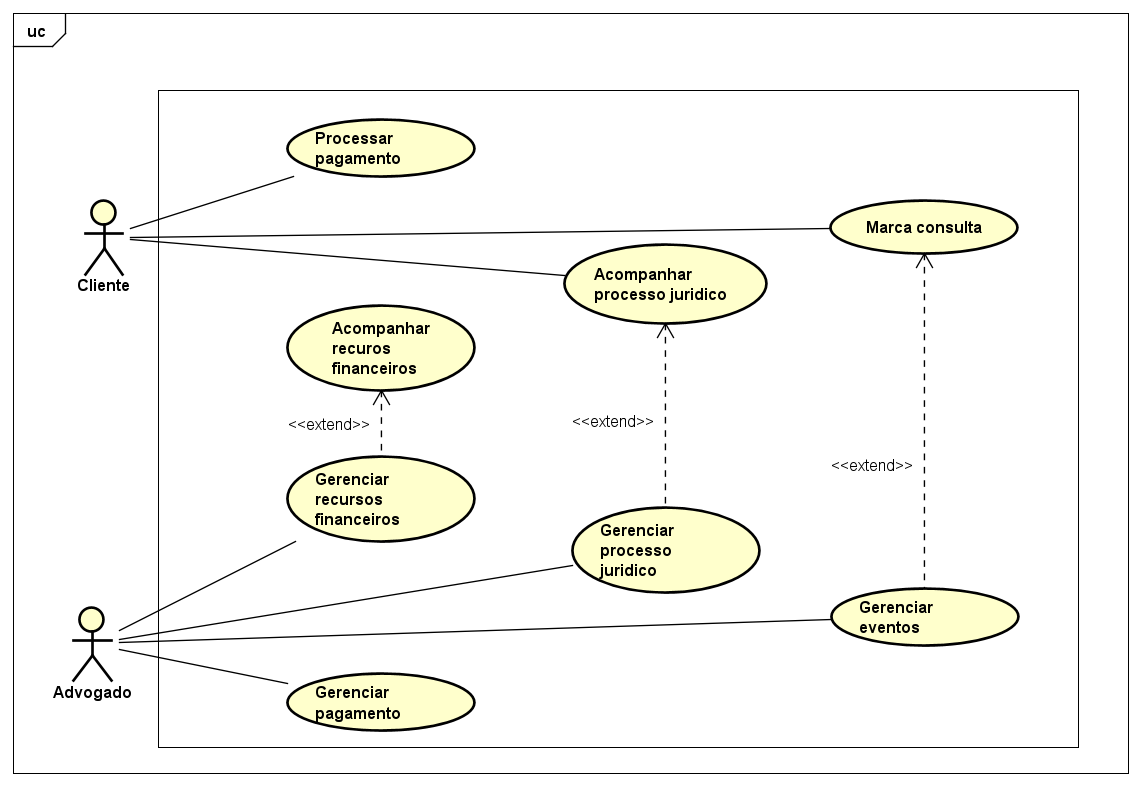
\includegraphics[width=0.8\linewidth]{imagens/Caso de uso MR Telles v5.png}
\end{figure}

Conforme detalhado na Figura 1, o ator Cliente e Advogado serão os únicos usuários ao
utilizar o sistema.
\begin{itemize}
    \item \textbf{Cliente}: Responsável por pagamentos, acompanhamento financeiro, seus processos e consultas.
    \item \textbf{Administrador (Advogado)}: Gerencia todas as funcionalidades do sistema.
\end{itemize}


\begin{enumerate}[leftmargin=*]
    \item \textbf{Processar Pagamento} (Cliente)
    \begin{itemize}
        \item Visualização de parcelas mensais
        \item Geração de QR Code PIX
        \item Confirmação manual pelo administrador
    \end{itemize}
    
    \item \textbf{Gerenciar Pagamento} (Administrador)
    \begin{itemize}
        \item Geração de PIX avulso para não cadastrados
        \item Identificação do pagador no histórico
        \item Armazenamento em lista de transações
    \end{itemize}

    \item \textbf{Acompanhar Recursos Financeiros} (Cliente)
    \begin{itemize}
        \item Visualização de parcelas pendentes
        \item Informações de valor, vencimento e status
        \item Acompanhamento de obrigações financeiras
    \end{itemize}

    \item \textbf{Gerenciar Recursos Financeiros} (Administrador)
    \begin{itemize}
        \item Cadastro de parcelas por cliente
        \item Atualização de status de pagamento
        \item Histórico financeiro
    \end{itemize}
    
    \item \textbf{Acompanhar Processo Jurídico} (Cliente)
    \begin{itemize}
        \item Consulta de andamentos processuais
        \item Visualização de histórico
        \item Detalhamento de etapas
    \end{itemize}
    
    \item \textbf{Gerenciar Processo Jurídico} (Administrador)
    \begin{itemize}
        \item Cadastro de novos processos
        \item Atualização de etapas
        \item Registro de decisões judiciais
    \end{itemize}
    
    \item \textbf{Marcar Consulta} (Cliente)
    \begin{itemize}
        \item Agendamento por calendário interativo
        \item Seleção de horários disponíveis
        \item Cancelamento de agendamentos
    \end{itemize}
    
    \item \textbf{Gerenciar Eventos} (Administrador)
    \begin{itemize}
        \item Controle completo de agenda
        \item Reagendamento de consultas
        \item Cadastro de eventos internos
    \end{itemize}
\end{enumerate}


\newpage
\section{Diagrama de Classes}\label{sec:diagrama-classes}

Na Figura \ref{fig:16}, observa-se a definição de seis classes principais para o sistema MR Telles. As classes \texttt{User}, \texttt{ControleFinanceiro}, \texttt{Processo} e \texttt{Schedule} concentram os relacionamentos centrais do sistema, compartilhando informações entre si e possibilitando a automação de funcionalidades jurídicas e financeiras.

As classes \texttt{Histórico} e \texttt{PhiTransaction} não se conectam diretamente a todas as entidades, mas são essenciais para garantir o registro de ações e a flexibilidade no controle de transações. Além disso, o diagrama representa os vínculos como associação, agregação e composição entre as classes, oferecendo suporte à rastreabilidade, gestão processual e controle de eventos.


\begin{figure}[!ht]
    \centering
    \caption{Diagrama de Classe}
    \label{fig:16}
    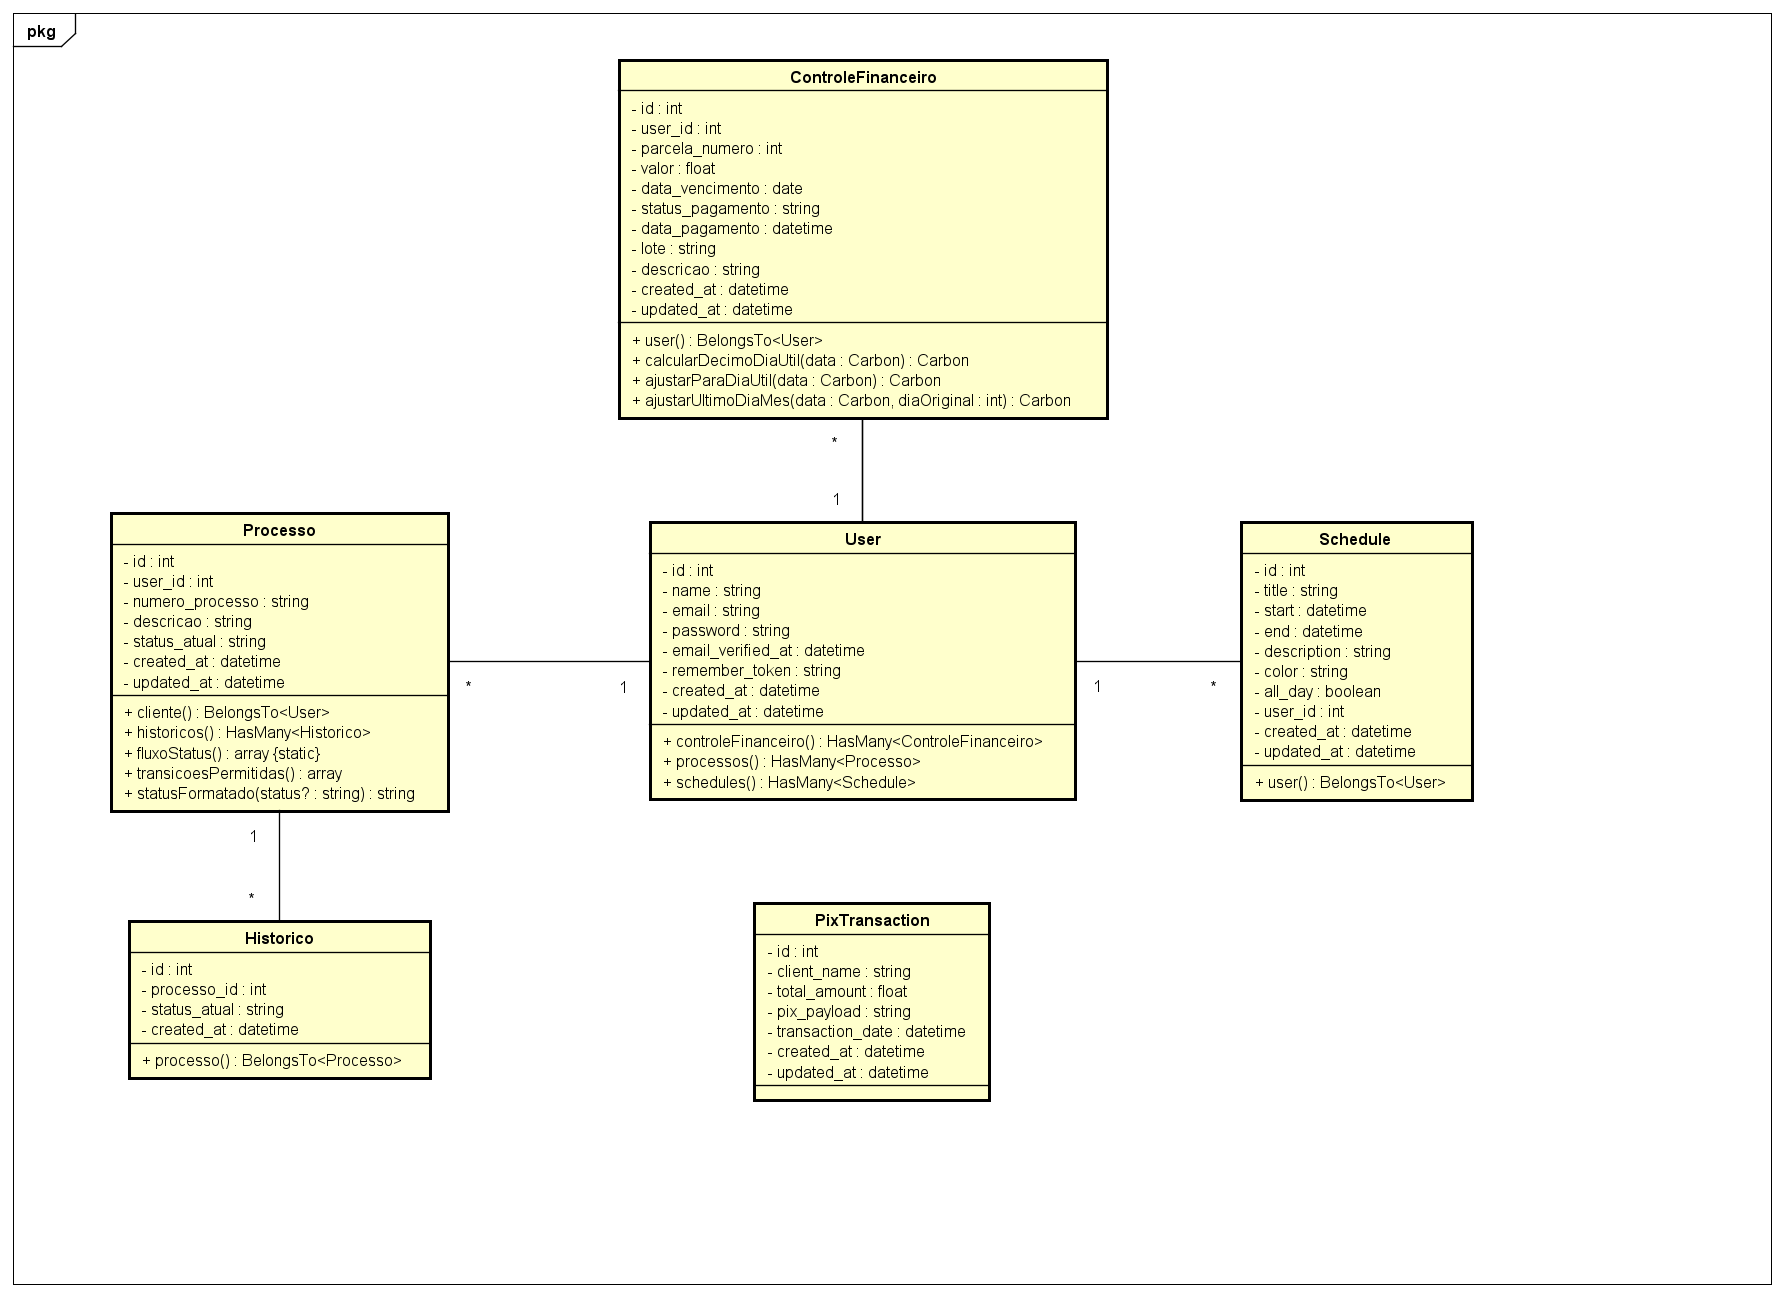
\includegraphics[width=0.8\linewidth]{imagens/uml/diagrama de classe MR Telles.png}
\end{figure}


\newpage
\section{Diagrama Entidade Relacionamento}
Na Figura \ref{fig:17}, é apresentado o diagrama entidade relacionamento (DER) é uma representação gráfica que descreve a estrutura de um banco de dados, mostrando entidades, atributos e relacionamentos. Ele é usado para modelar dados, facilitando o entendimento e o design do esquema de banco de dados. O DER do sistema MR Telles, que ilustra a estrutura do banco de dados. As principais entidades incluem users, controle financeiro, processos, historicos, schedules e pix transactions list. A entidade users está no centro da estrutura, relacionando-se diretamente com o controle financeiro, processos jurídicos e agendamento de eventos.

\begin{figure}[!ht]
    \centering
    \caption{Diagrama Entidade Relacionamento}
    \label{fig:17}
    \includegraphics[width=0.8\linewidth]{imagens/uml/Der.png}
\end{figure}

\newpage
\section{Diagrama de Implantação}
Na Figura \ref{fig:18}, o diagrama de implantação do sistema MR Telles apresenta uma arquitetura cliente-servidor convencional, onde a aplicação web é hospedada no serviço de cloud InfinityFree, executando-se sobre um sistema operacional genérico. Os usuários acessam o sistema através de navegadores web (browsers) em suas máquinas locais, que se comunicam com o servidor via protocolos TCP/IP pela internet. O armazenamento de dados é gerenciado pelo SGBD MySQL, que opera em conjunto com a aplicação web para persistência das informações.

\begin{figure}[!ht]
    \centering
    \caption{Diagrama de Implantação}
    \label{fig:18}
    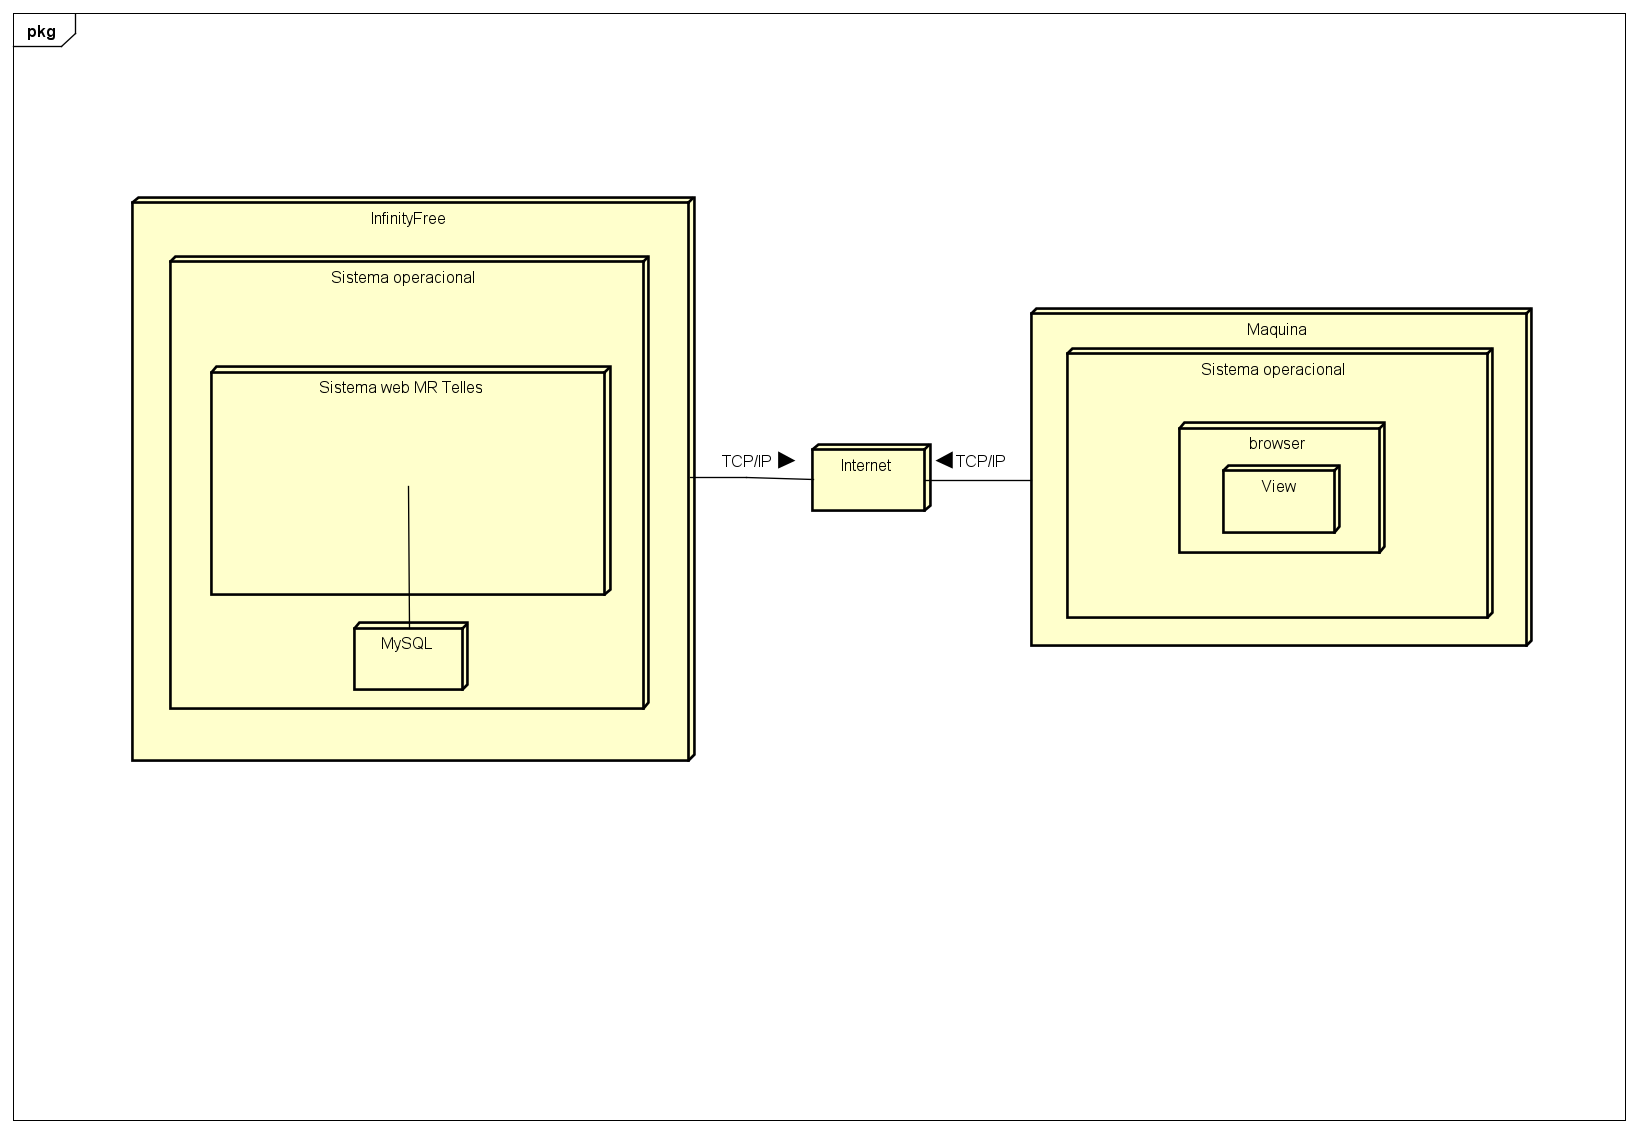
\includegraphics[width=0.8\linewidth]{imagens/uml/diagrama de implantação.png}
\end{figure}

\section{Diagrama de Sequência}
O diagrama de sequência é uma representação gráfica que descreve como objetos interagem em um cenário específico, mostrando a ordem das mensagens trocadas entre eles ao longo do tempo. Utilizado na modelagem de comportamento, ele ajuda a visualizar a dinâmica do fluxo de controle e comunicação em um sistema.


\subsection{Diagrama de Sequencia Gerenciar Eventos}

Na Figura \ref{fig:19} o administrador gerencie a agenda do escritório por meio de um calendário interativo:

\begin{itemize} \item Ao acessar a página inicial, o calendário é carregado com todos os eventos armazenados no banco de dados. \item O administrador pode adicionar novos eventos preenchendo um formulário com informações como título, data, descrição e cor. \item Eventos existentes podem ser editados diretamente via um modal interativo, com atualizações sendo salvas por requisições AJAX. \item A exclusão de eventos também ocorre via modal, com confirmação e remoção imediata do calendário. \end{itemize}
Esse fluxo é dinamicamente atualizado no frontend com o uso da biblioteca \texttt{FullCalendar}, mantendo a sincronização com os dados persistidos no backend.


\subsection{Diagrama de Sequencia Marcar Consulta}

Na Figura \ref{fig:20} o cliente agenda consultas jurídicas por meio de um formulário interativo:

\begin{itemize} \item Ao acessar a página, o cliente visualiza um formulário e uma tabela com suas consultas já marcadas. \item Ao selecionar uma data, o sistema consulta os horários disponíveis para aquele dia, excluindo os já ocupados. \item O cliente escolhe o horário e preenche as informações da consulta, que é registrada no sistema após envio do formulário. \item A consulta recém-criada aparece na lista do cliente e os horários são atualizados dinamicamente. \item O cliente também pode excluir consultas anteriores, com a atualização automática da agenda. 
\end{itemize}
Esse fluxo garante controle total do agendamento por parte do cliente, com sincronização em tempo real via AJAX.

\subsection{Diagrama de Sequencia Gerenciar Pagamento}

Na Figura \ref{fig:21} o administrador gere cobranças via QR Code PIX, mesmo para clientes que não estão cadastrados no sistema:

\begin{itemize} \item O administrador acessa a interface de geração de PIX e visualiza um formulário para inserção do nome do cliente e valor a ser cobrado. \item Após o envio do formulário, o sistema gera automaticamente o payload PIX e seu respectivo QR Code utilizando a biblioteca \texttt{BaconQrCode}. \item A transação gerada é registrada no banco de dados e adicionada à lista de histórico visível na mesma página. \item O administrador pode também excluir transações anteriores diretamente da lista, com atualização imediata da interface. \end{itemize}
Este fluxo permite manter um controle prático e histórico de cobranças avulsas, sem necessidade de vínculo direto com um usuário autenticado.

\subsection{Diagrama de Sequencia Processar Pagamento}

Na Figura \ref{fig:22} o cliente visualize e pague suas parcelas pendentes referentes ao mês atual:

\begin{itemize} \item Ao acessar a página de pagamento, o sistema filtra e exibe apenas as parcelas pendentes do cliente no mês vigente. \item Para cada parcela exibida, o cliente pode clicar em "Gerar Pagamento", acionando a geração de um QR Code PIX. \item O sistema valida a autorização de acesso à parcela, gera o payload conforme o padrão Pix e exibe o QR Code para pagamento. \item O cliente deve então realizar o pagamento manualmente usando seu aplicativo bancário. \item Após o pagamento, o administrador deve confirmar manualmente no sistema através da funcionalidade \textit{Gerenciar Recursos Financeiros}. \end{itemize}

Este fluxo não possui automação de confirmação de pagamento, funcionando com validação visual por parte do administrador.

\subsection{Diagrama de Sequencia Acompanhar Processo Jurídico}

Na Figura \ref{fig:23} o cliente pode consultar o andamento de seus processos jurídicos cadastrados no sistema:

\begin{itemize} \item O cliente acessa a página de processos, onde é exibida uma lista com todos os processos atribuídos a ele, incluindo número, descrição, status atual e data da última atualização. \item Ao clicar em "Ver Detalhes", o cliente é redirecionado para uma tela com informações completas do processo selecionado. \item Nessa visualização detalhada, são exibidos os dados do processo e um histórico cronológico das etapas, com seus respectivos status e datas. \end{itemize}

Essa funcionalidade visa dar transparência ao cliente sobre o andamento de seu processo jurídico, sem interferência administrativa.

\subsection{Diagrama de Sequencia Gerenciar Processo Jurídico}
Na Figura \ref{fig:24} o administrador realizar a gestão completa dos processos jurídicos dos clientes:

\begin{itemize} \item Ao acessar a tela de processos, o administrador visualiza a lista de processos com filtros e informações básicas. \item É possível cadastrar um novo processo preenchendo o formulário com o número, cliente e descrição. O status inicial é registrado automaticamente como "protocolado". \item Cada processo pode ter o status atualizado manualmente, com registro da data da mudança, criando um histórico completo de movimentações. \item O administrador também pode excluir processos, o que remove tanto o processo quanto seu histórico associado. \end{itemize}

Essa funcionalidade fornece uma visão completa e controlada da evolução dos processos jurídicos do escritório.


\begin{figure}[!ht]
    \centering
    \caption{Diagrama de Sequencia Gerenciar Eventos}
    \label{fig:19}
    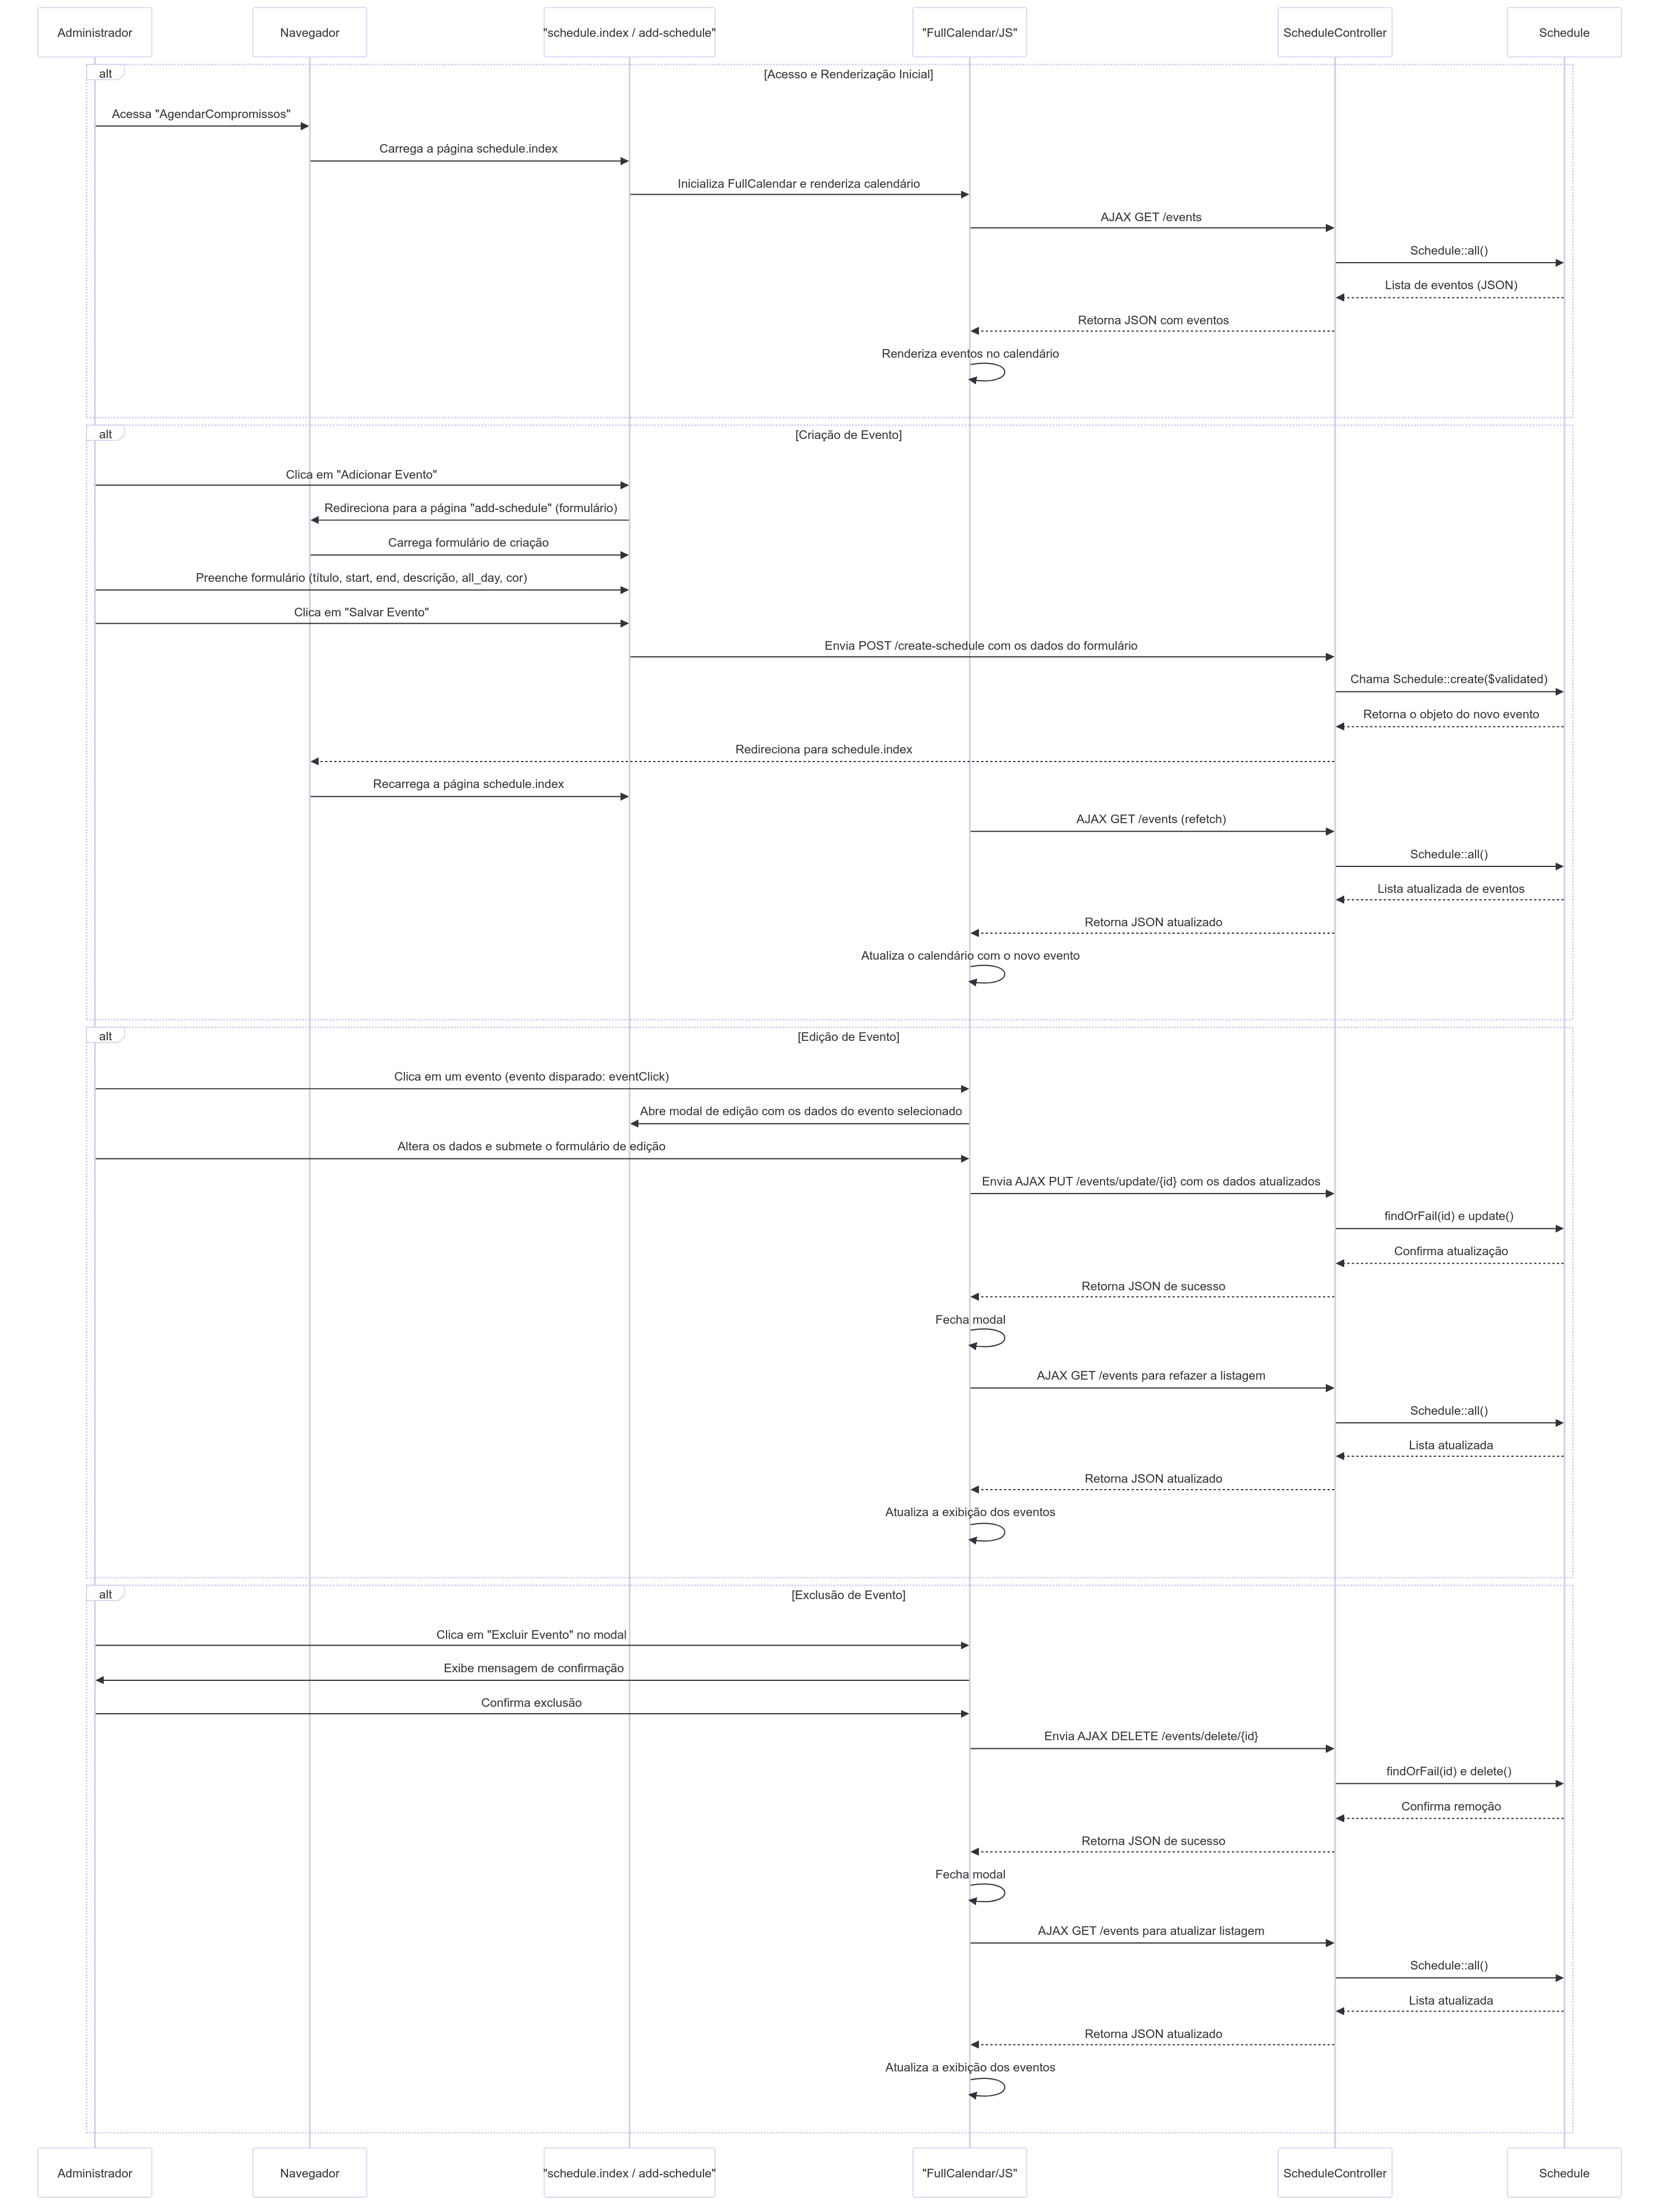
\includegraphics[width=0.8\linewidth]{imagens/uml/Diagrama de sequencia gerenciar eventos (1).png}
\end{figure}

\begin{figure}[!ht]
    \centering
    \caption{Diagrama de Sequencia Marcar Consulta}
    \label{fig:20}
    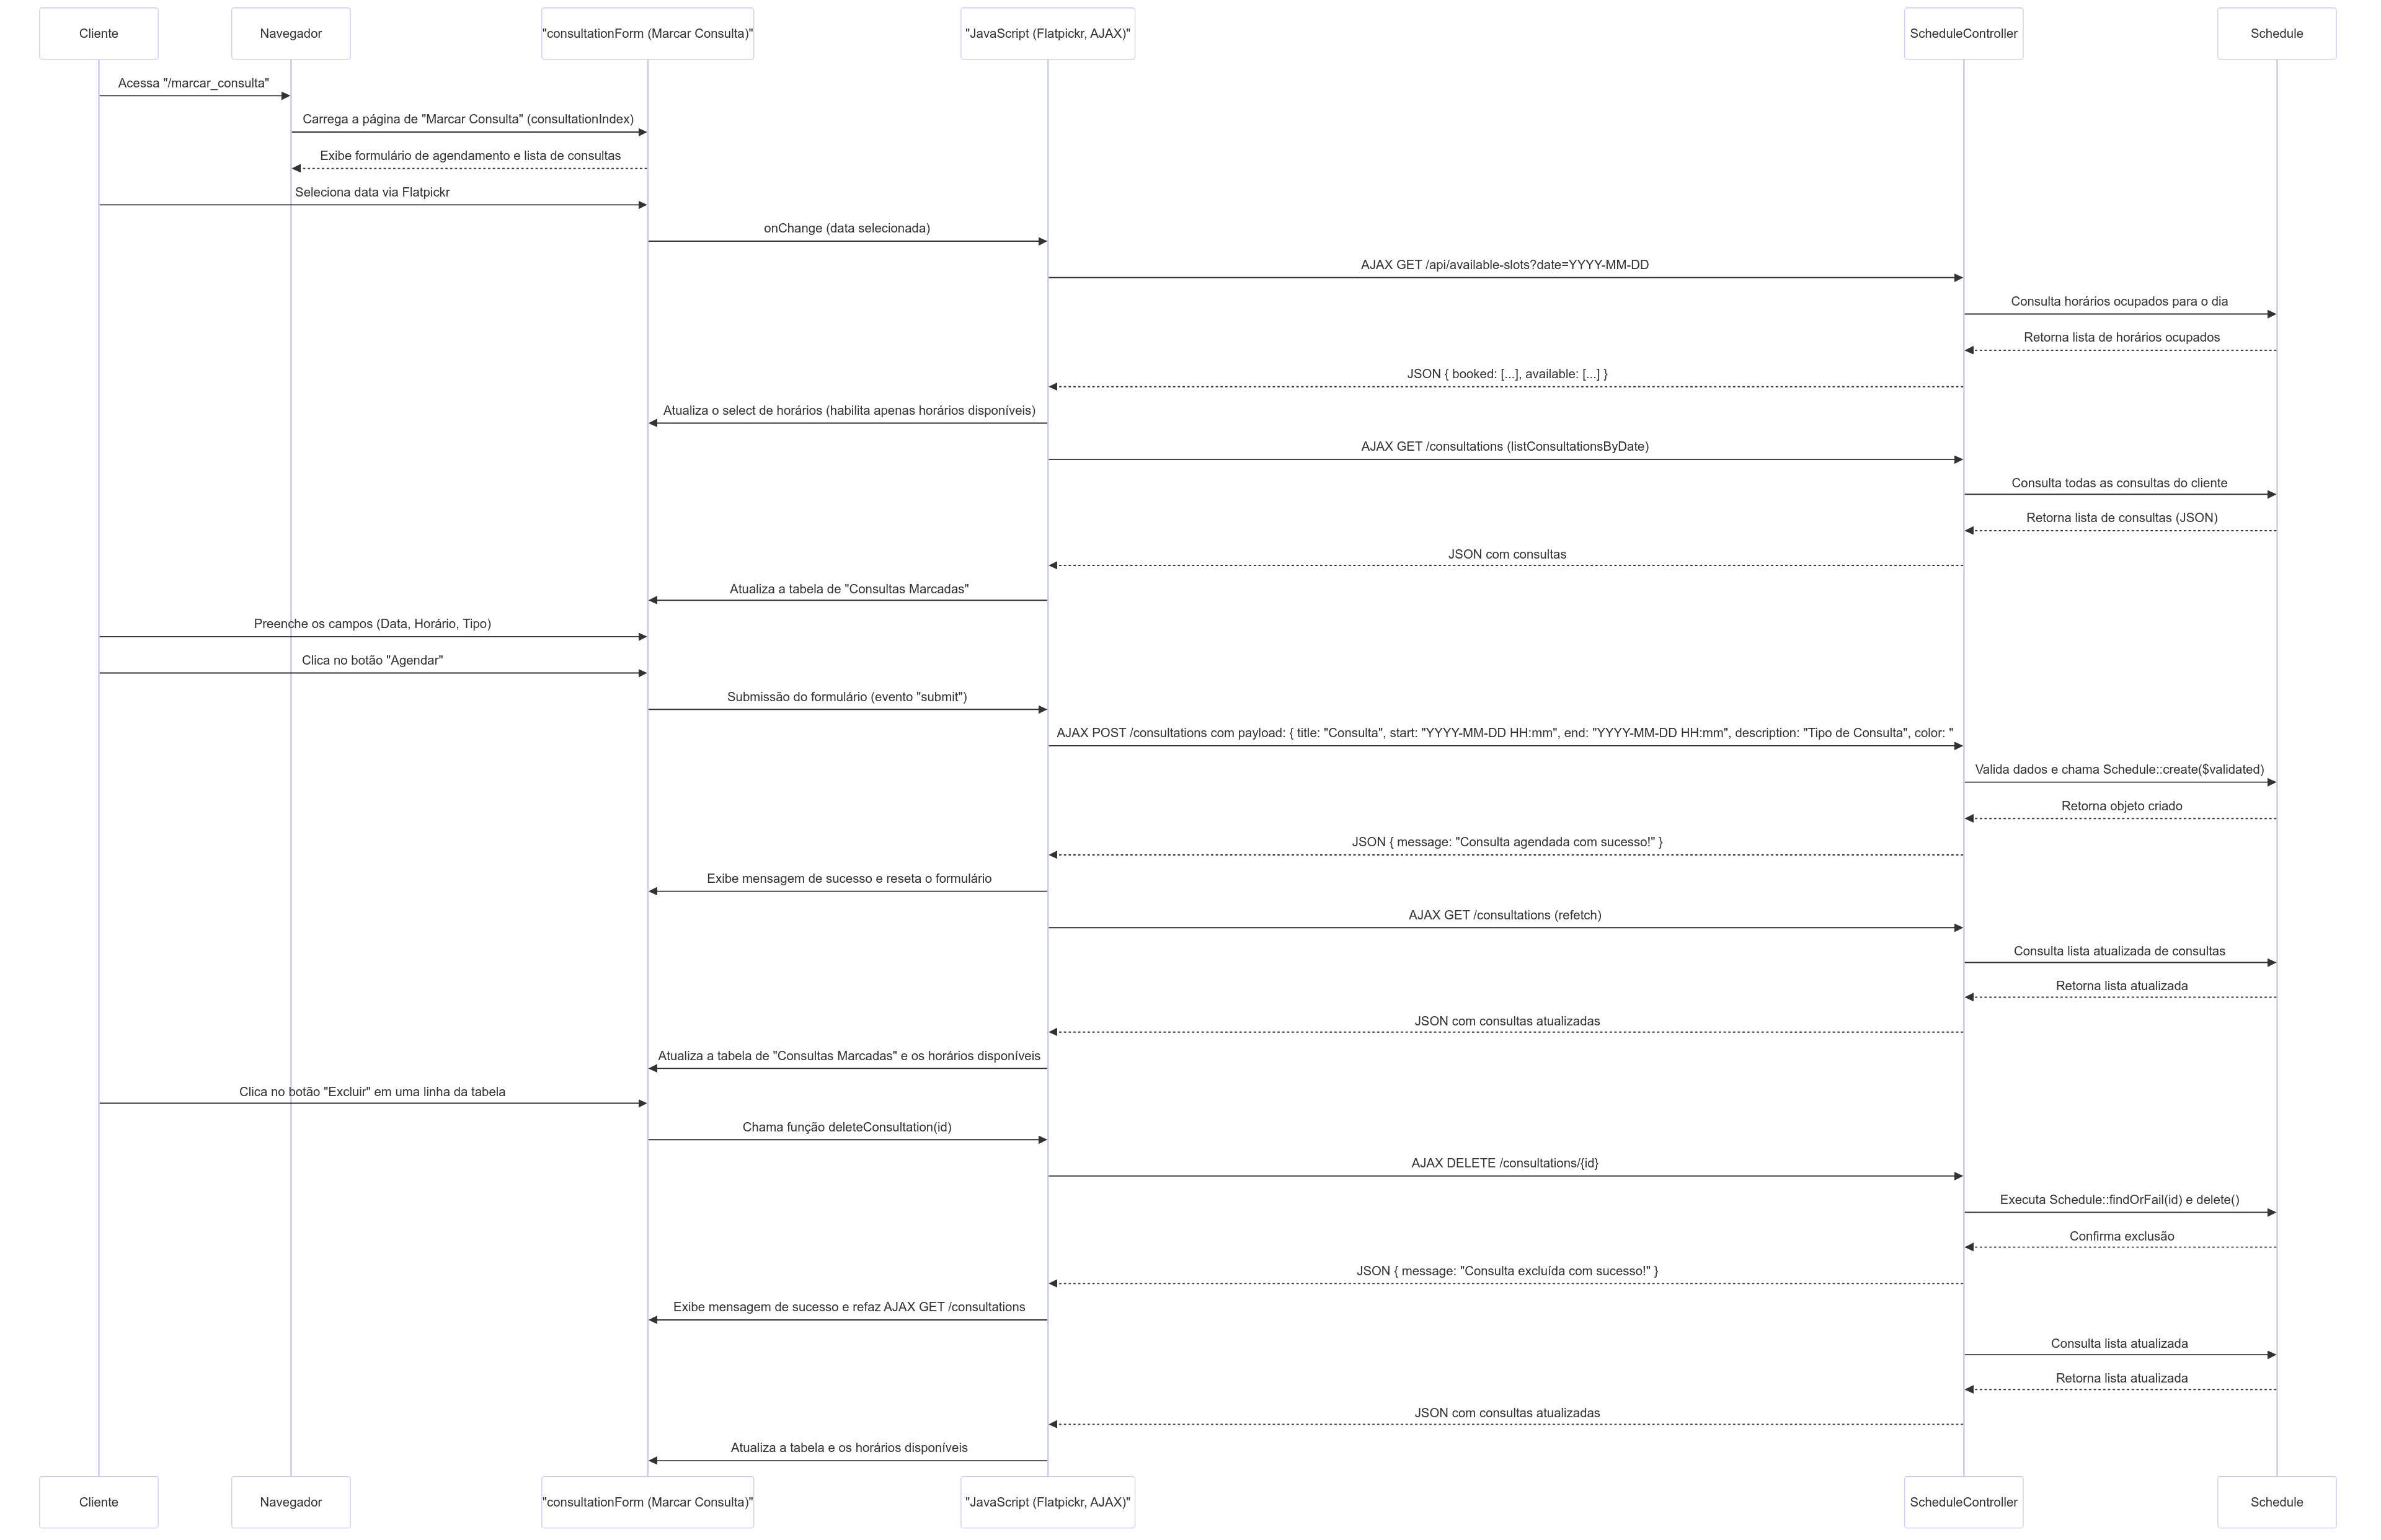
\includegraphics[width=0.8\linewidth]{imagens/uml/Diagrama de sequencia Marcar consulta (1).png}
\end{figure}

\begin{figure}[!ht]
    \centering
    \caption{Diagrama de Sequencia Gerenciar Pagamento}
    \label{fig:21}
    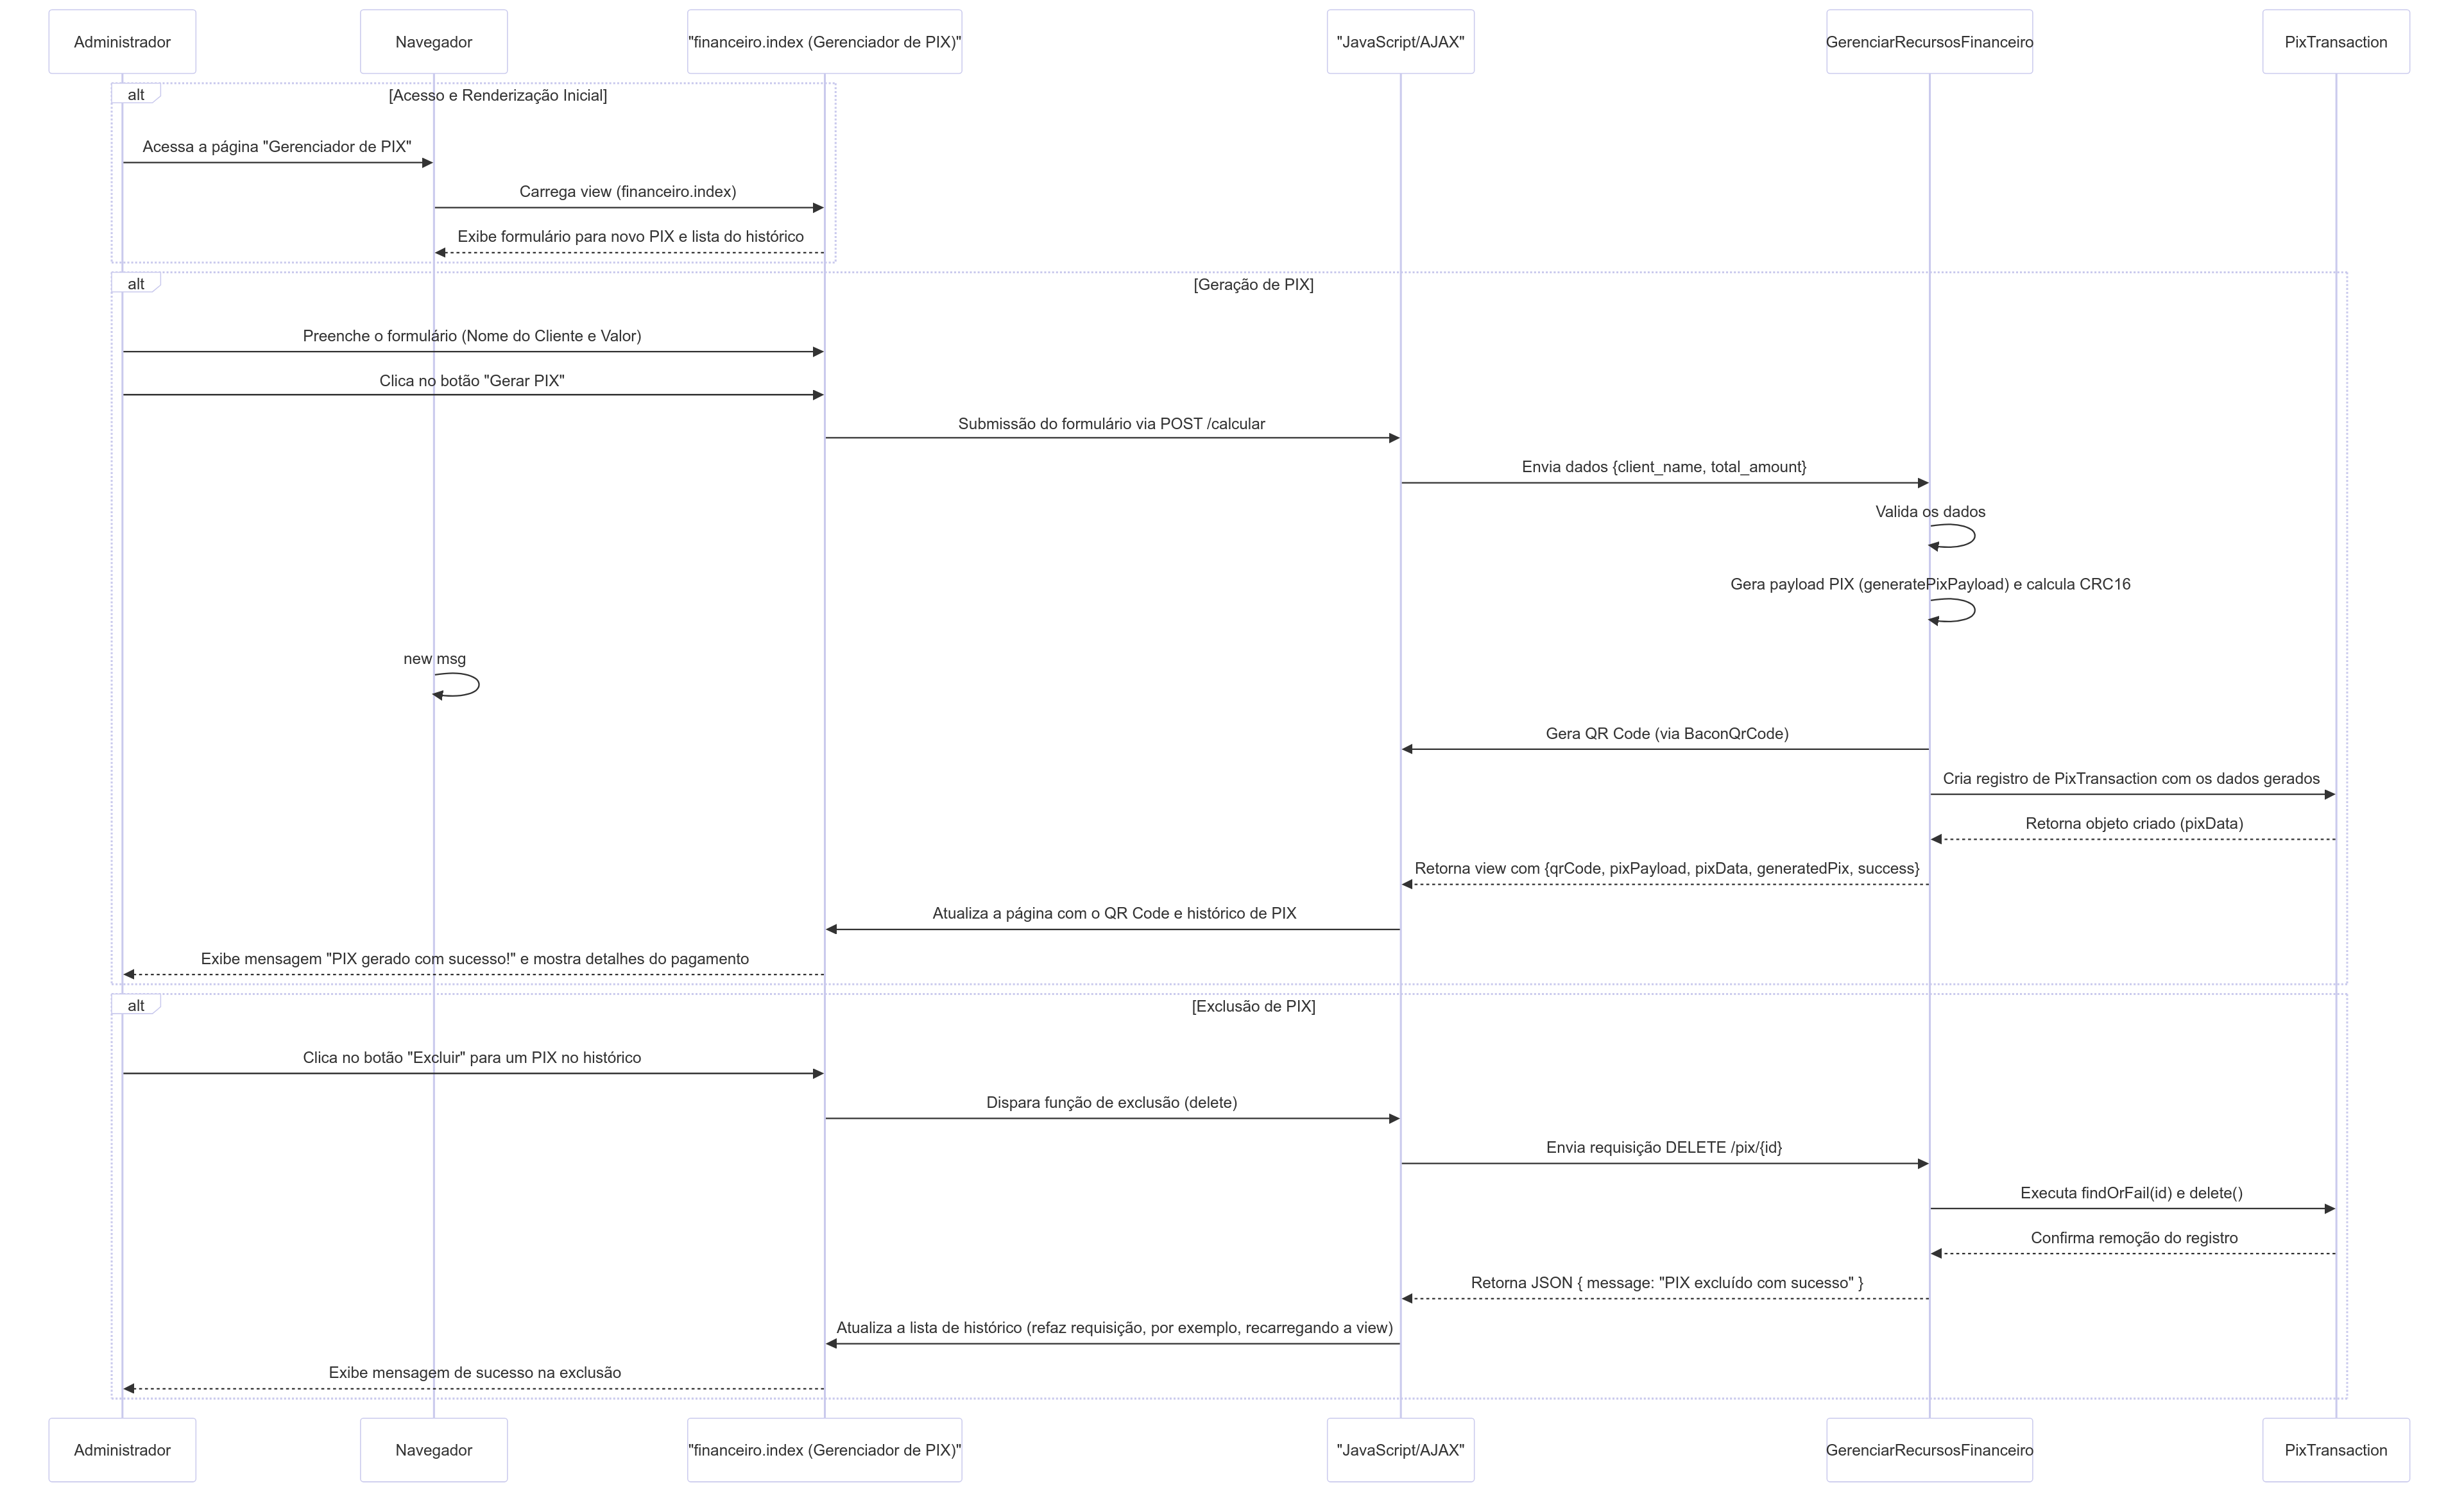
\includegraphics[width=0.8\linewidth]{imagens/uml/Diagrama de sequencia gerenciar Pagamento.png}
\end{figure}

\begin{figure}[!ht]
    \centering
    \caption{Diagrama de Sequencia Processar Pagamento}
    \label{fig:22}
    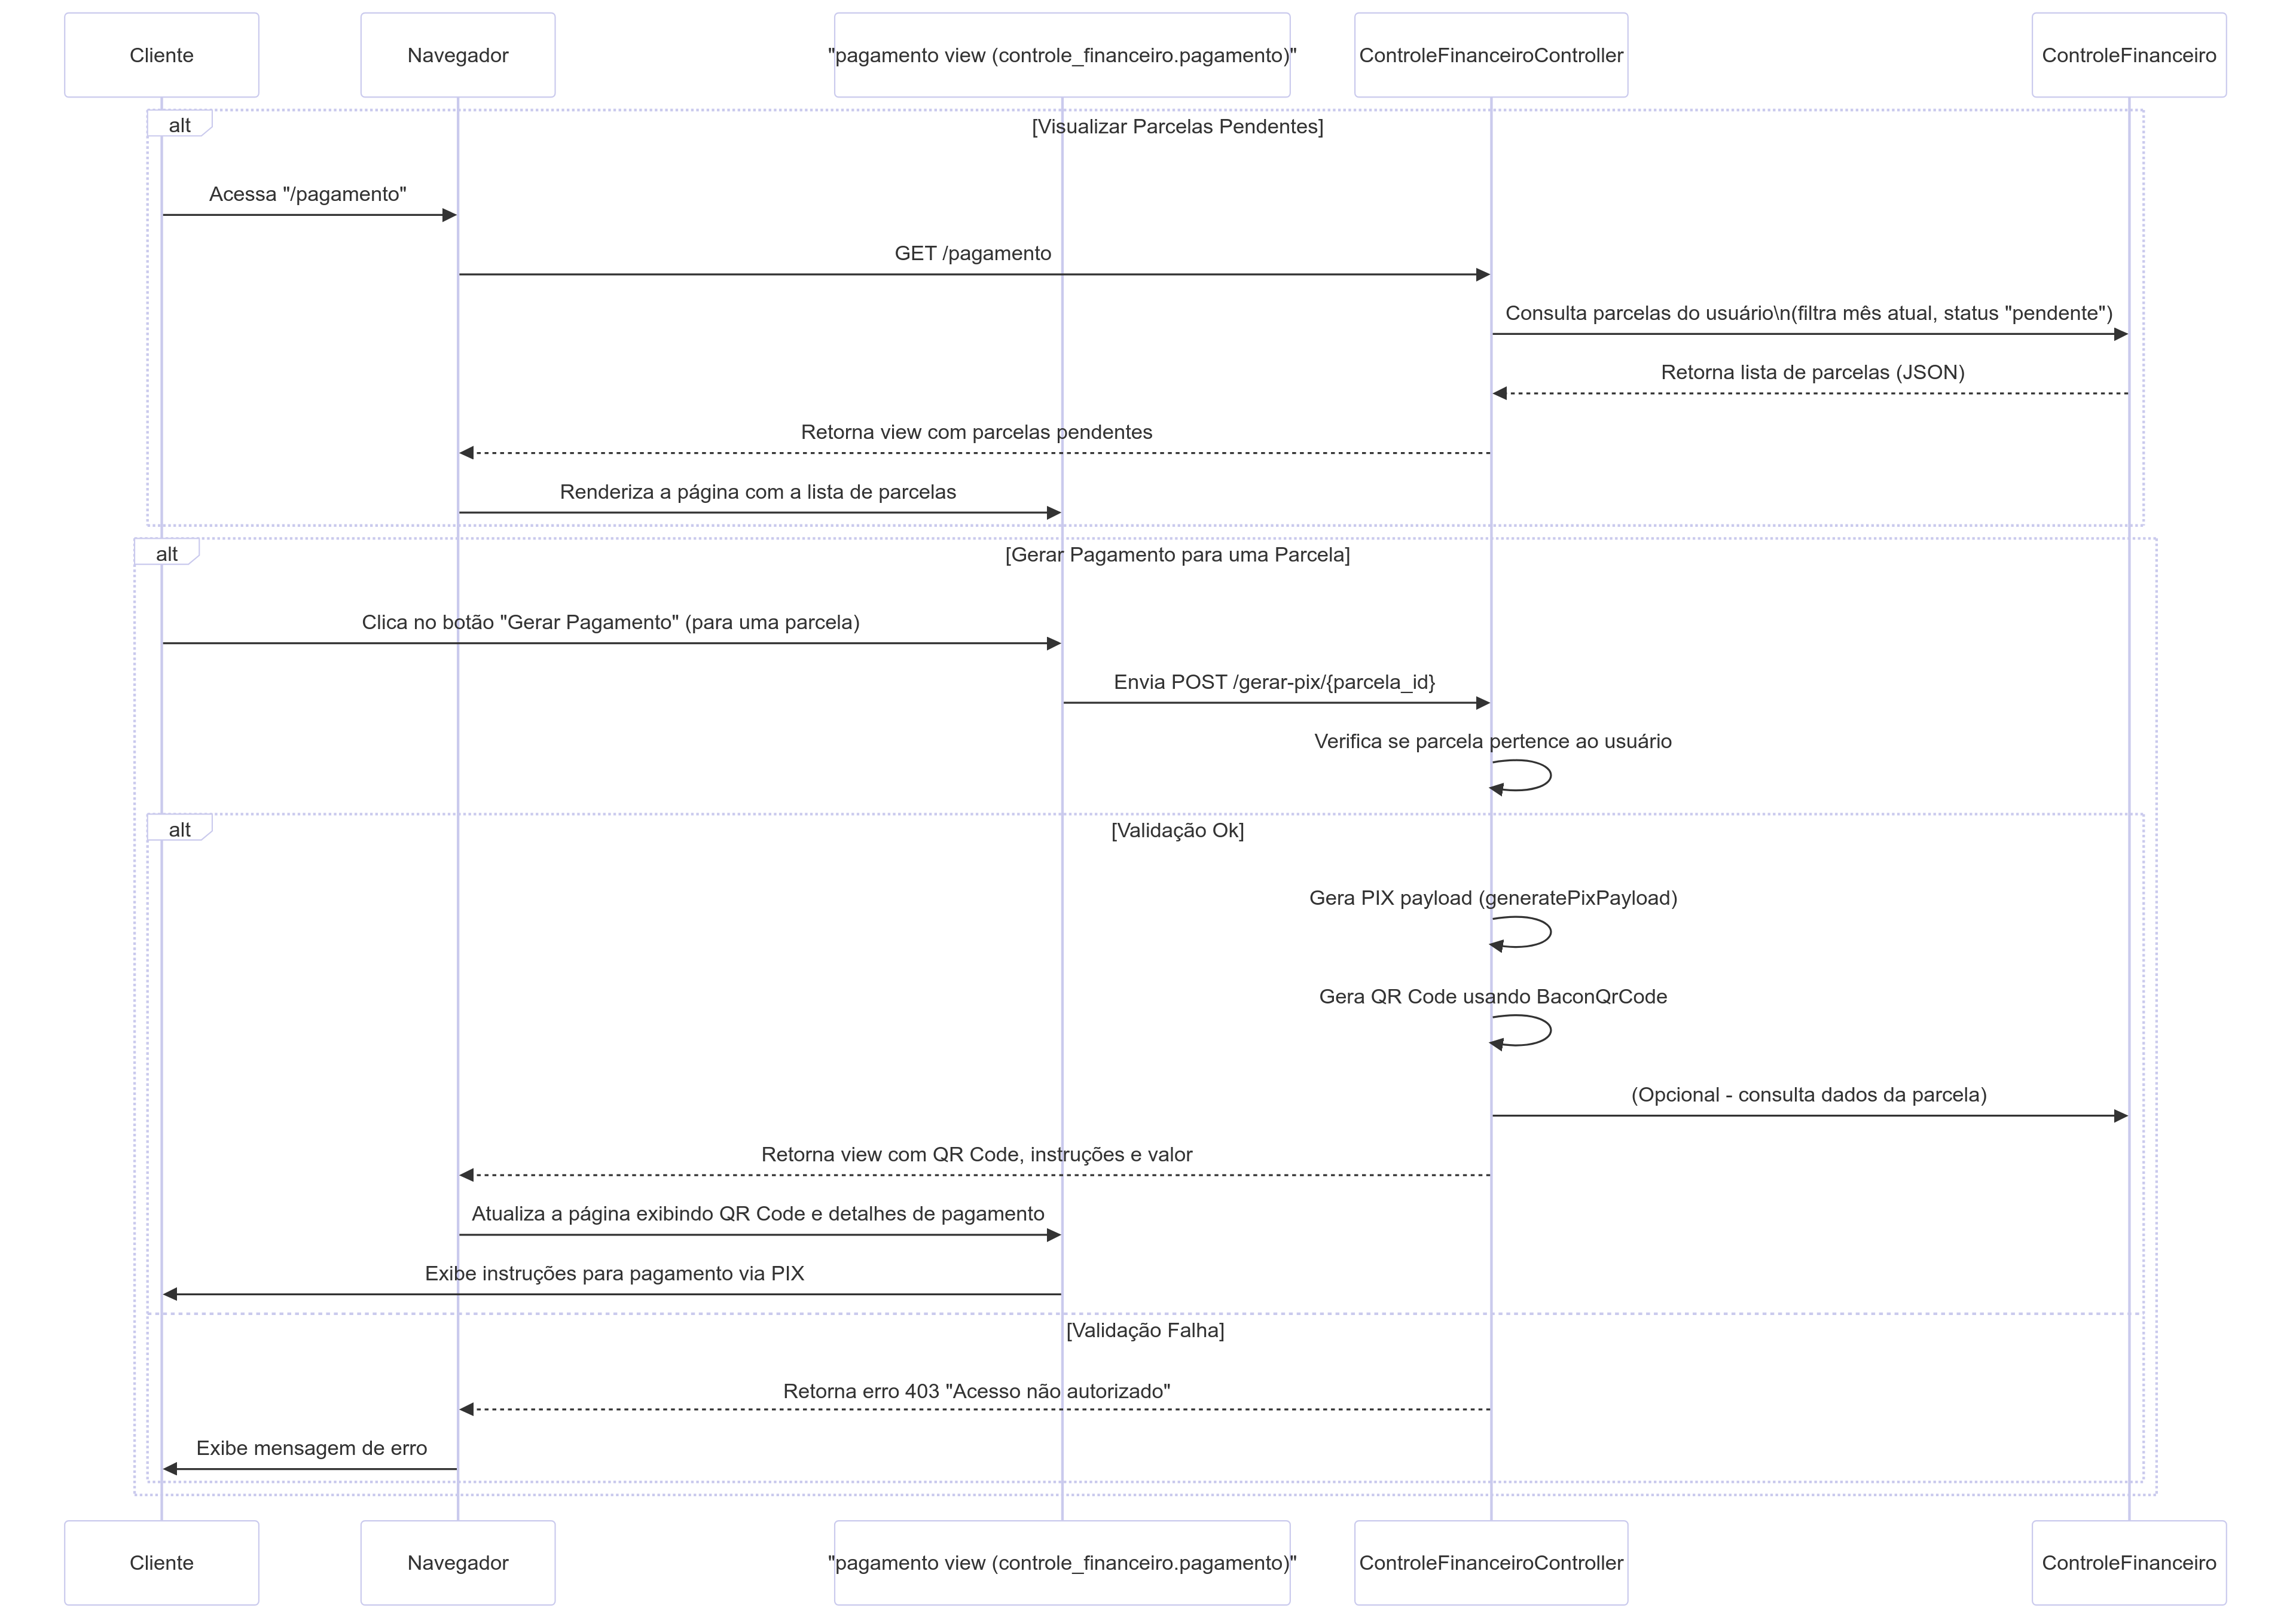
\includegraphics[width=0.8\linewidth]{imagens/uml/Diagrama de sequencia ProcessarPagamento (1).png}
\end{figure}

\begin{figure}[!ht]
    \centering
    \caption{Diagrama de Sequencia Acompanhar Processo Jurídico}
    \label{fig:23}
    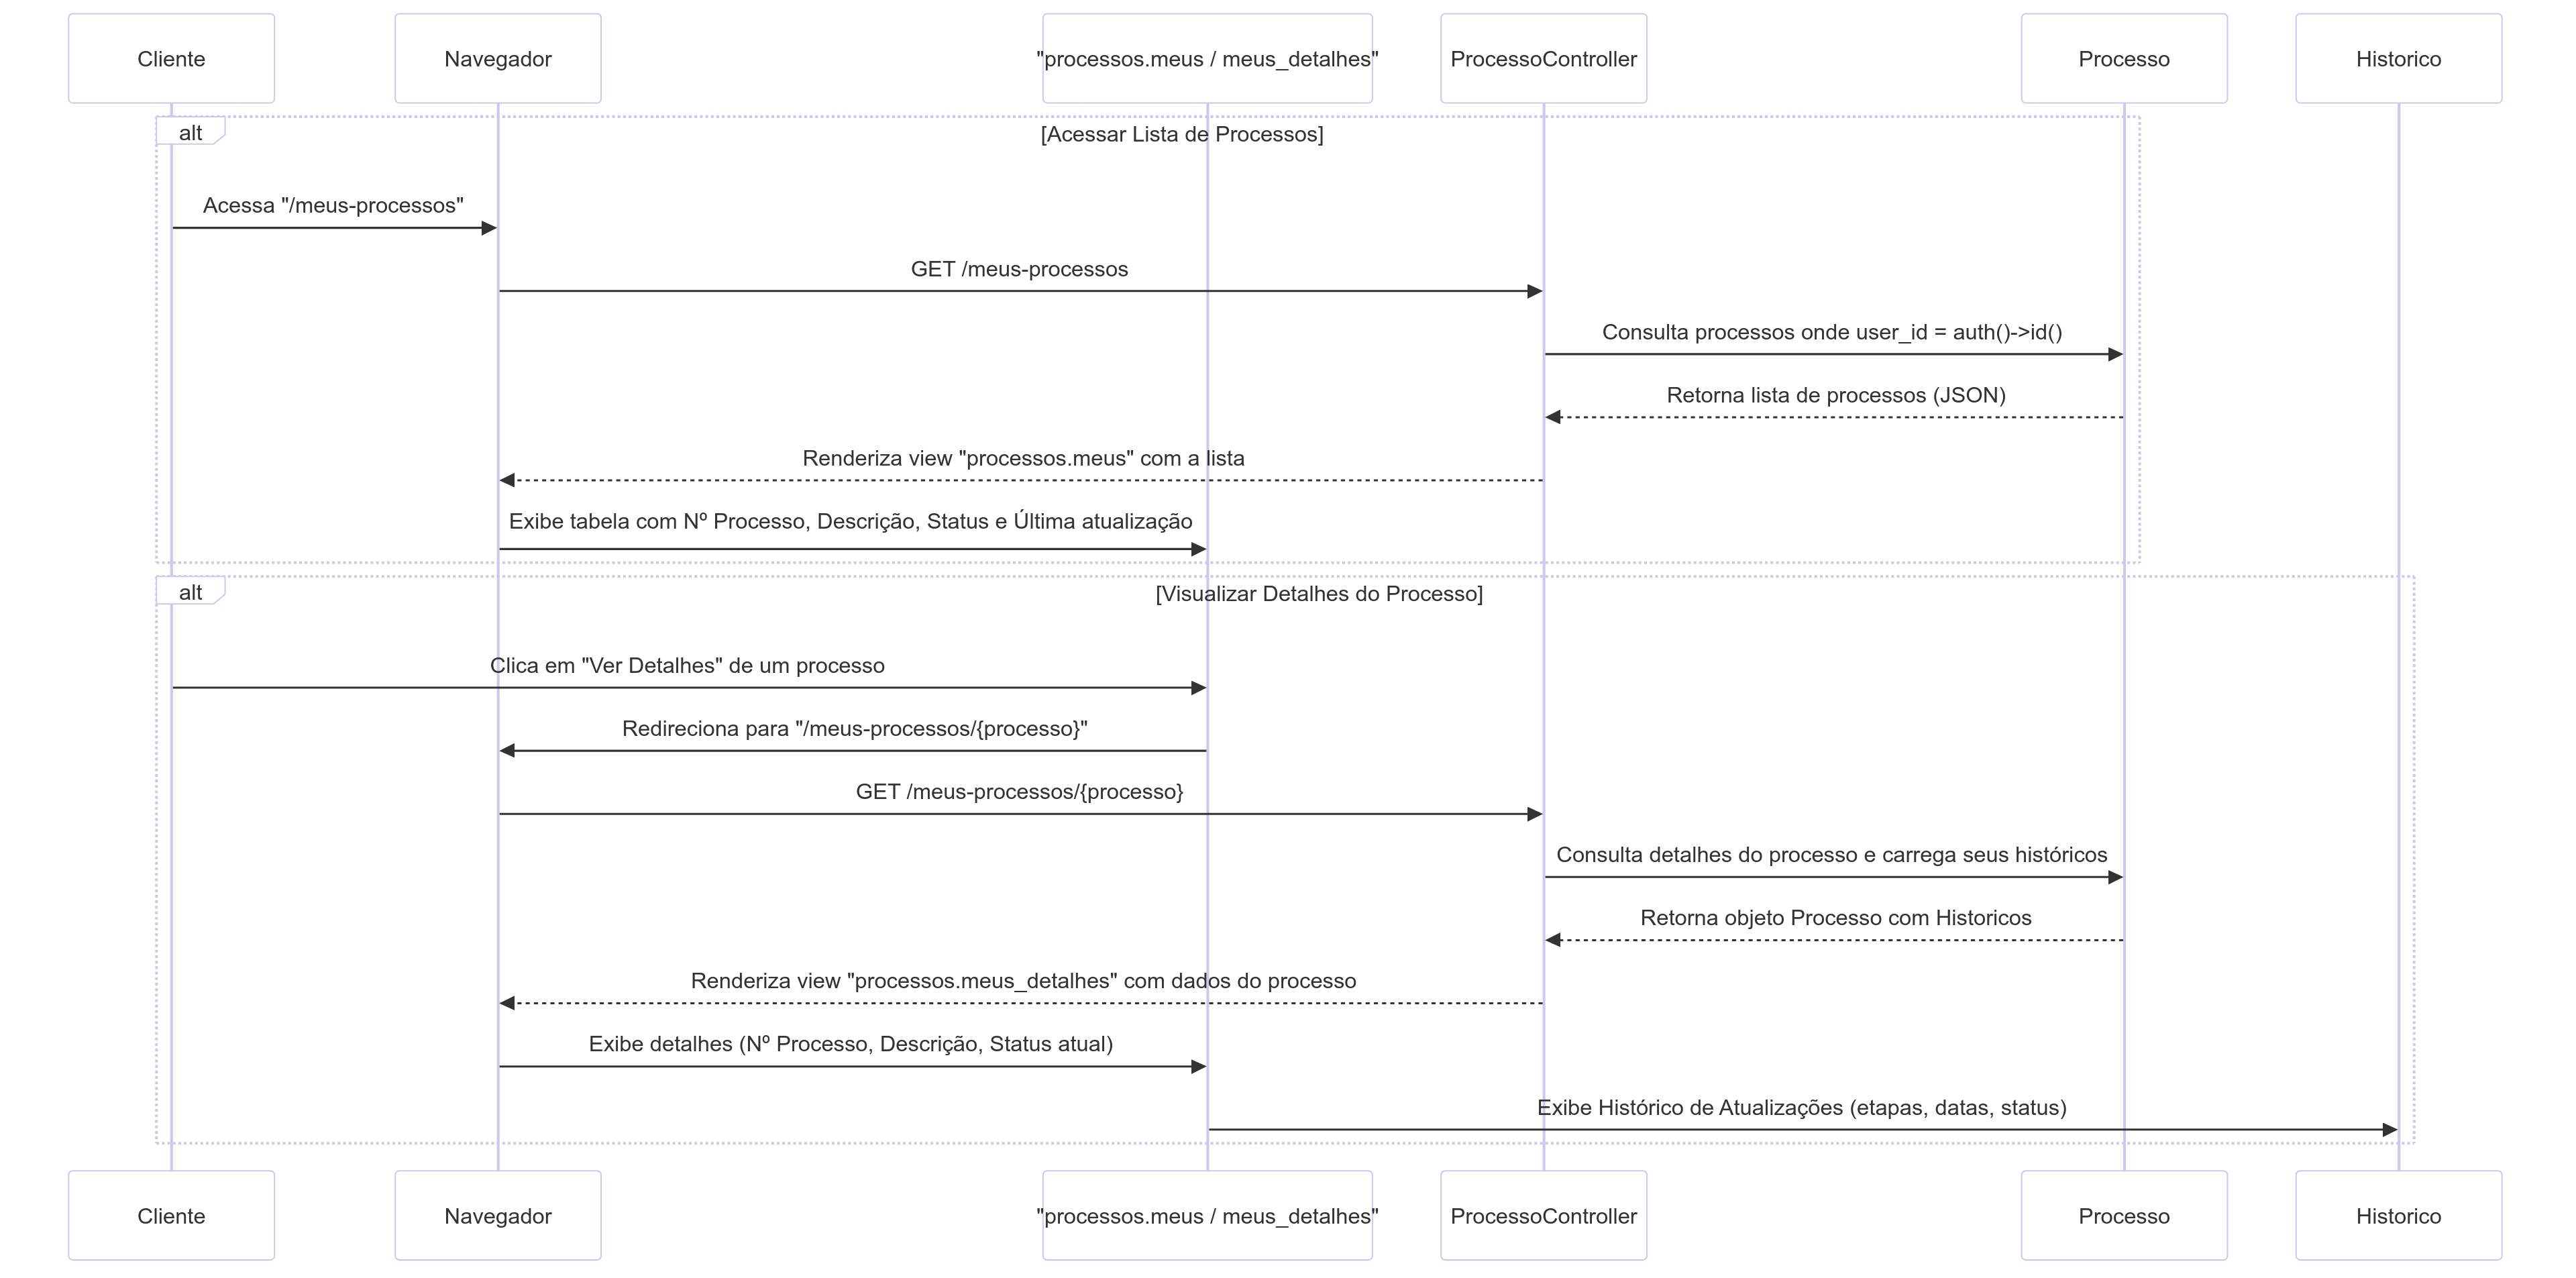
\includegraphics[width=0.8\linewidth]{imagens/uml/Diagrama de sequencia acompanhar processo juridico (1).png}
\end{figure}

\begin{figure}[!ht]
    \centering
    \caption{Diagrama de Sequencia Gerenciar Processo Jurídico}
    \label{fig:24}
    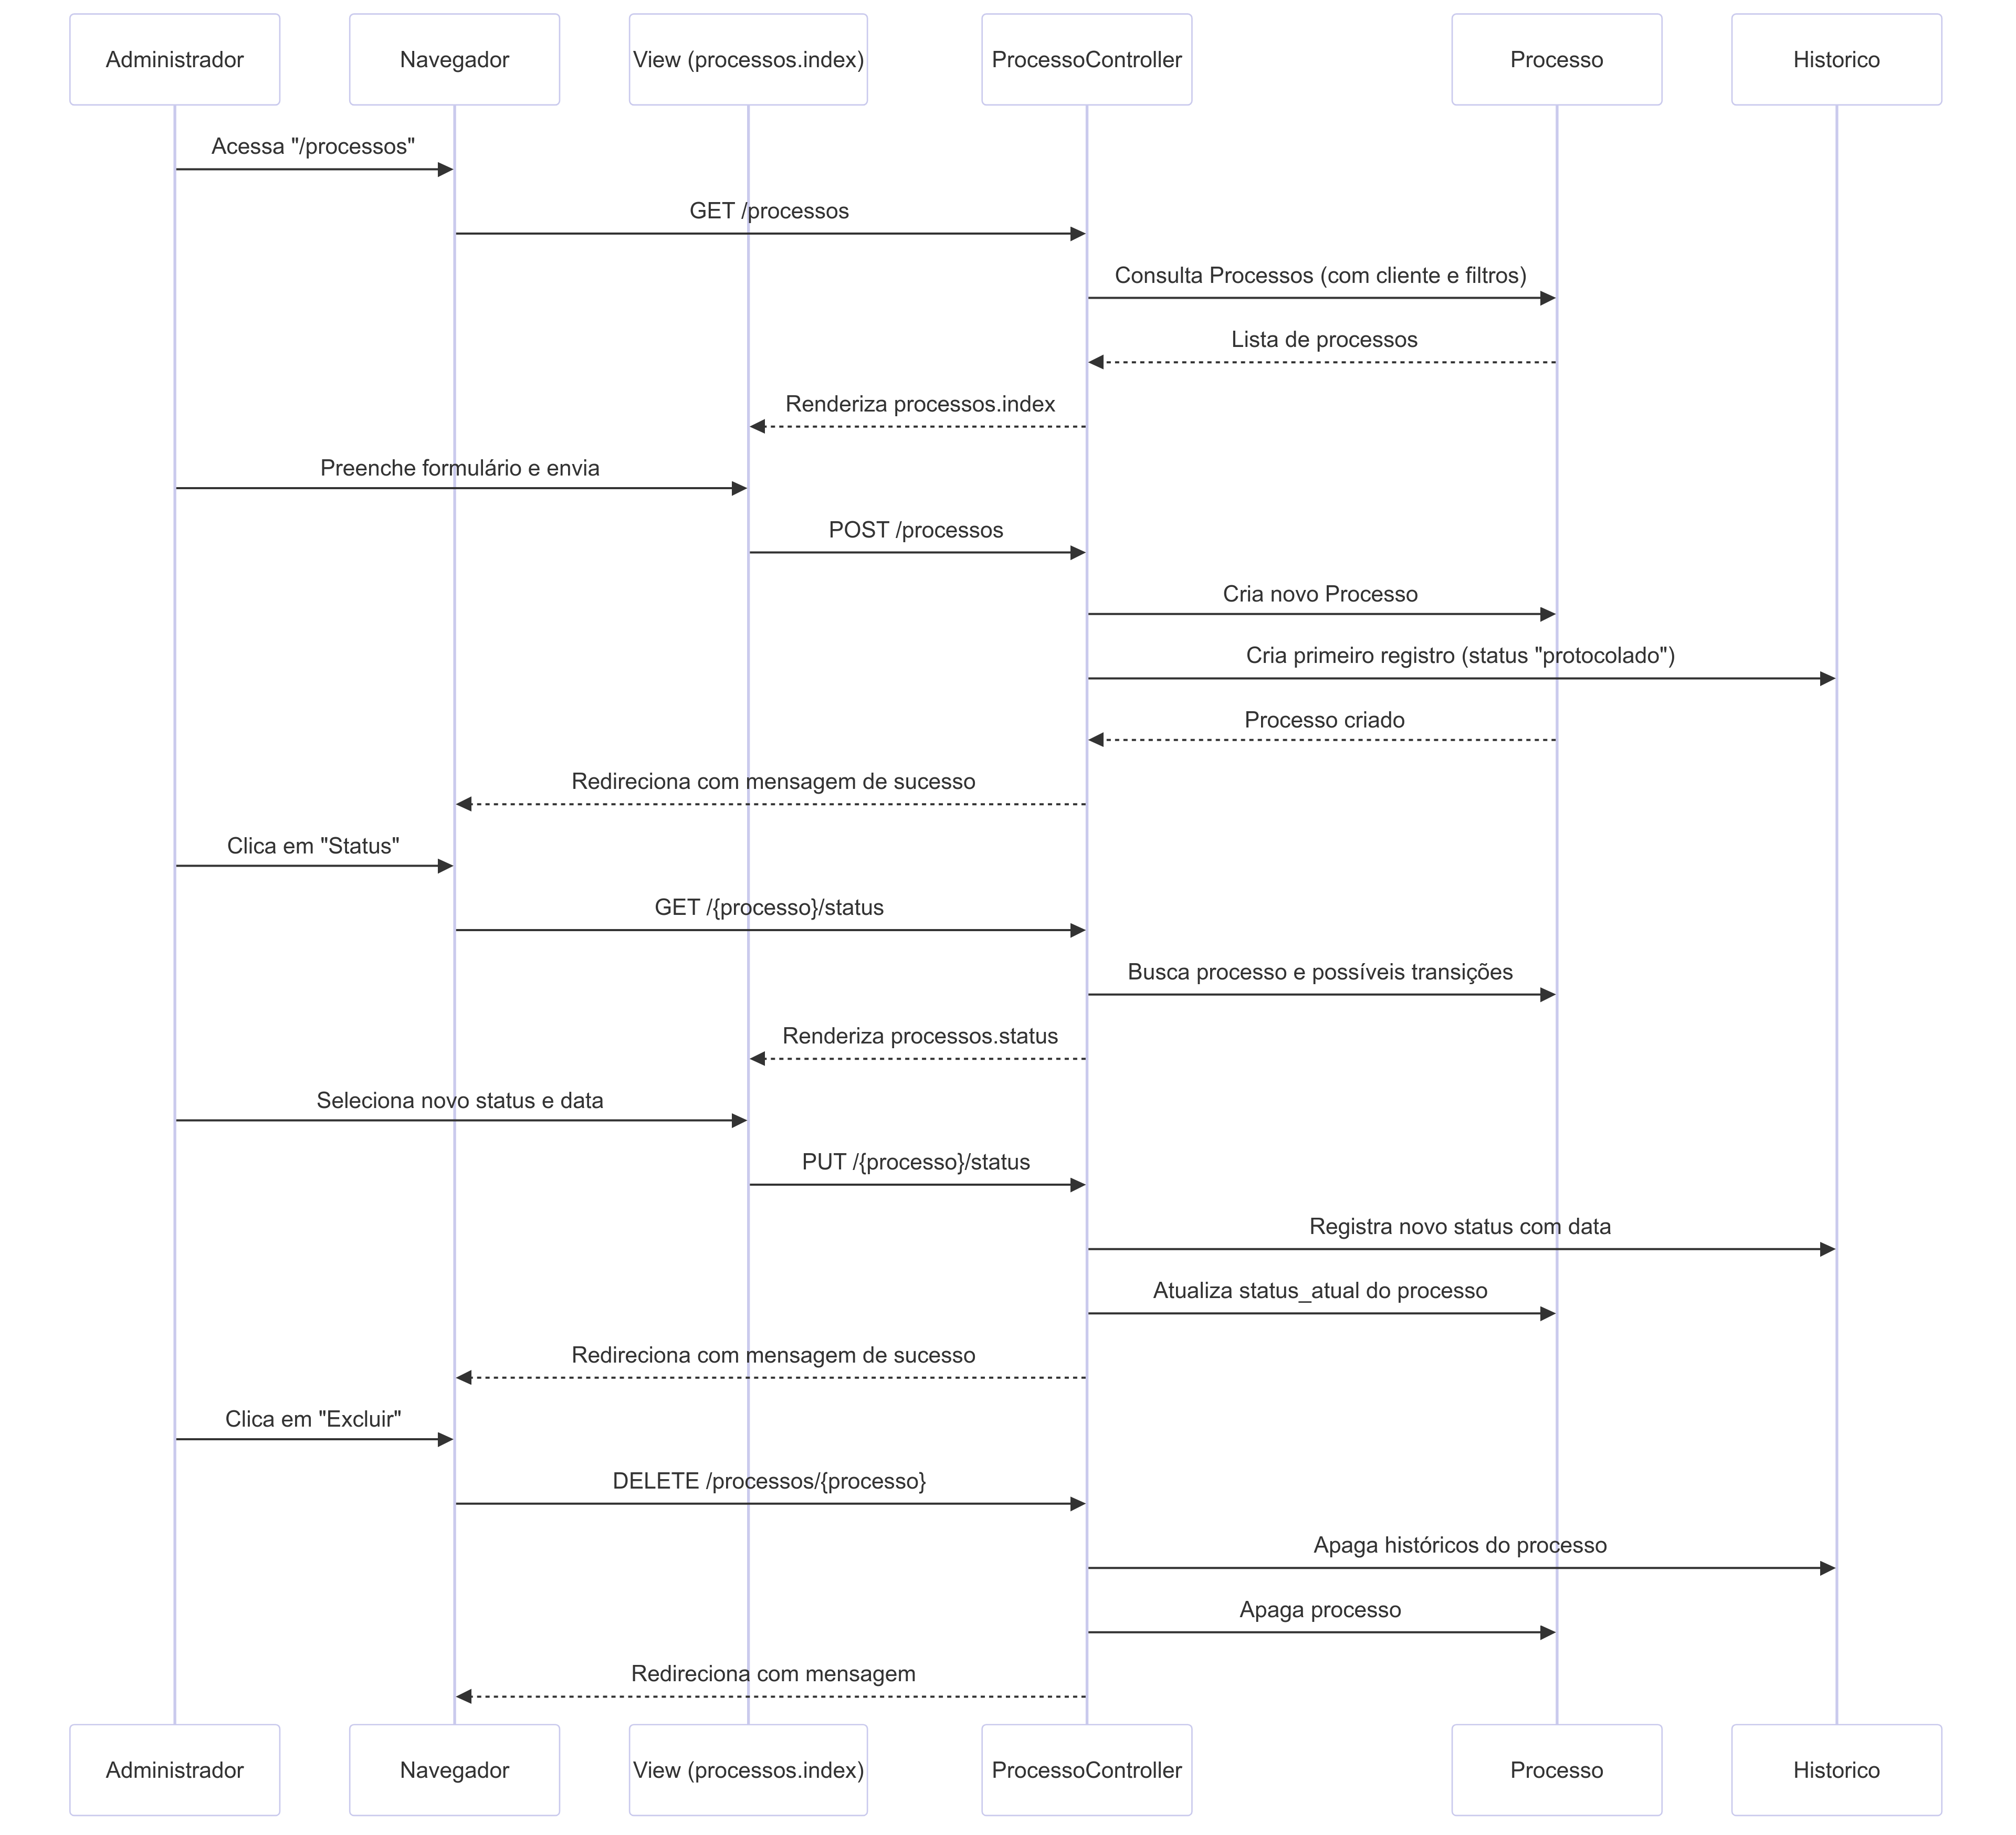
\includegraphics[width=0.8\linewidth]{imagens/uml/Diagrama de sequencia gerenciar processo juridico (1).png}
\end{figure}
\chapter{Workflow (as is) na notação BPMN}\label{sec:3}

Workflow (as is), na notação BPMN (Business Process Model and Notation), é uma representação gráfica de um processo de negócio conforme ele é atualmente executado. Ele descreve as atividades, decisões, eventos e fluxos de informações que ocorrem durante a realização de uma tarefa ou conjunto de tarefas dentro de uma organização. O objetivo do Workflow (as is) na notação BPMN é fornecer uma visão clara e detalhada do processo existente, destacando os pontos de entrada, saída, decisões e interações entre os elementos do processo. Isso permite uma compreensão completa e precisa do fluxo de trabalho atual, facilitando a identificação de áreas de melhoria e otimização.


Na Figura \ref{fig:11} , é apresentado o BPMP (as is) do gerenciamento de agendamento, onde mostra os processos de como os clientes fazem os agendamentos de suas consultas atualmente.

Na Figura \ref{fig:12}, é apresentado o BPMP (as is) do gerenciamento de compromissos, onde mostra os processos de como o advogado da MR Telles atualmente gerencia seus processos.

Na Figura \ref{fig:13}, é apresentado o BPMP (as is) do gerenciamento de processos, onde os clientes procuram o advogado para pedir informações sobre seus casos, tirar dúvidas e esclarecer qualquer mal-entendido durante o processo.

Na Figura \ref{fig:14}, é apresentado o BPMP (as is) do gerenciamento financeiro, onde mostra os processos de como o advogado da MR Telles gerencia suas demandas financeiras nas organizações e verifica seus valores.

Na Figura \ref{fig:15}, é apresentado o BPMP (as is) do gerenciamento de pagamento, onde mostra os processos de como o advogado da MR Telles gerencia suas demandas financeiras nas organizações, confere com o cliente, aplica desconto caso tenha sido negociado e, após isso, valida para passar ao cliente.


\begin{figure}
    \centering
    \caption{Agendamento-(as is)}
    \label{fig:11}
    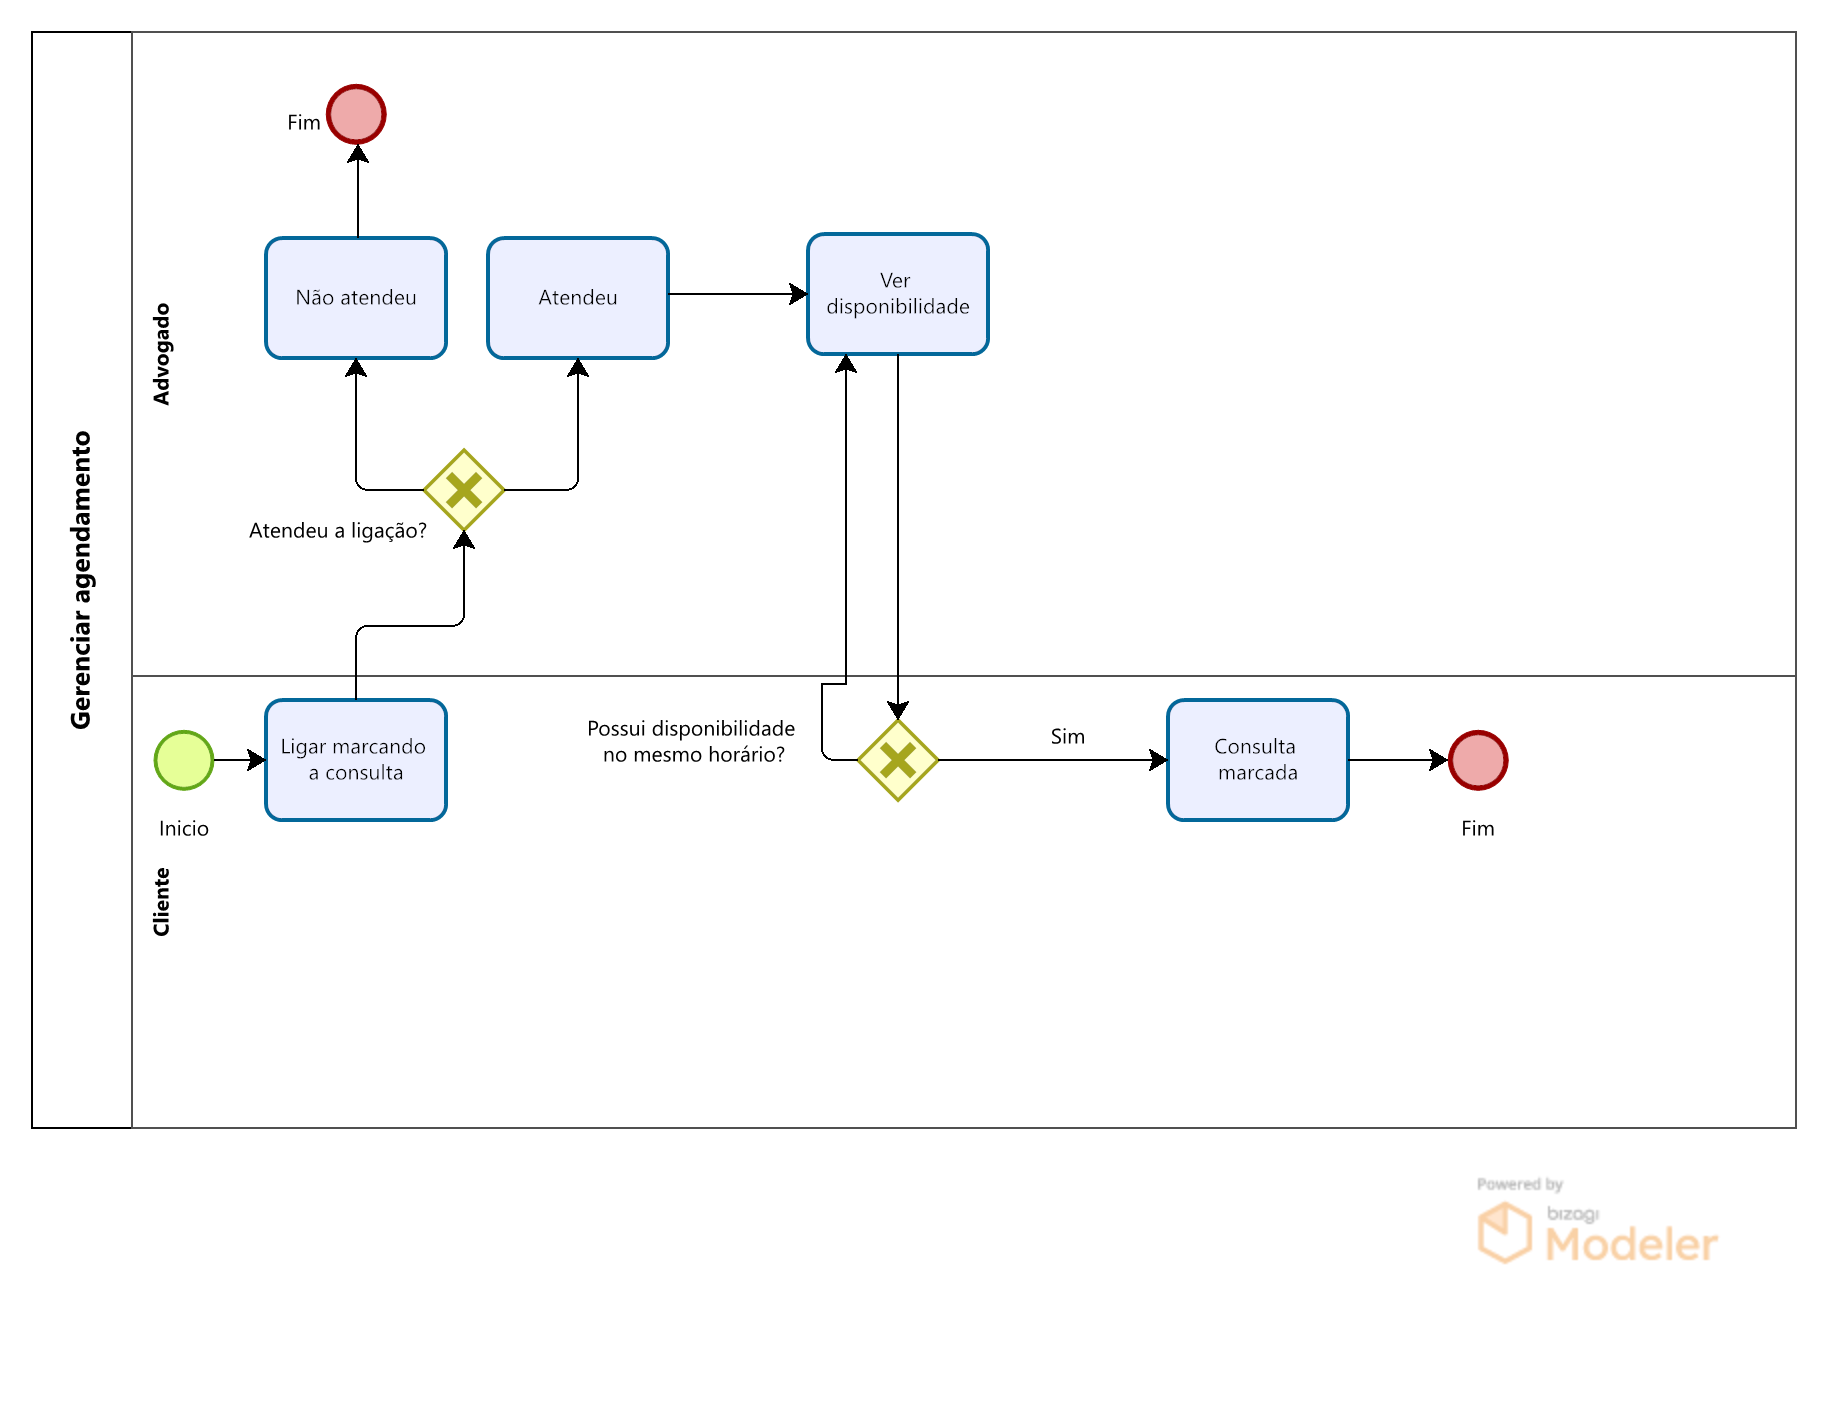
\includegraphics[width=0.8\linewidth]{imagens/BPMN/gerenciarAgendamento.png}
\end{figure}

\begin{figure}
    \centering
    \caption{Compromisso-(as is)}
    \label{fig:12}
    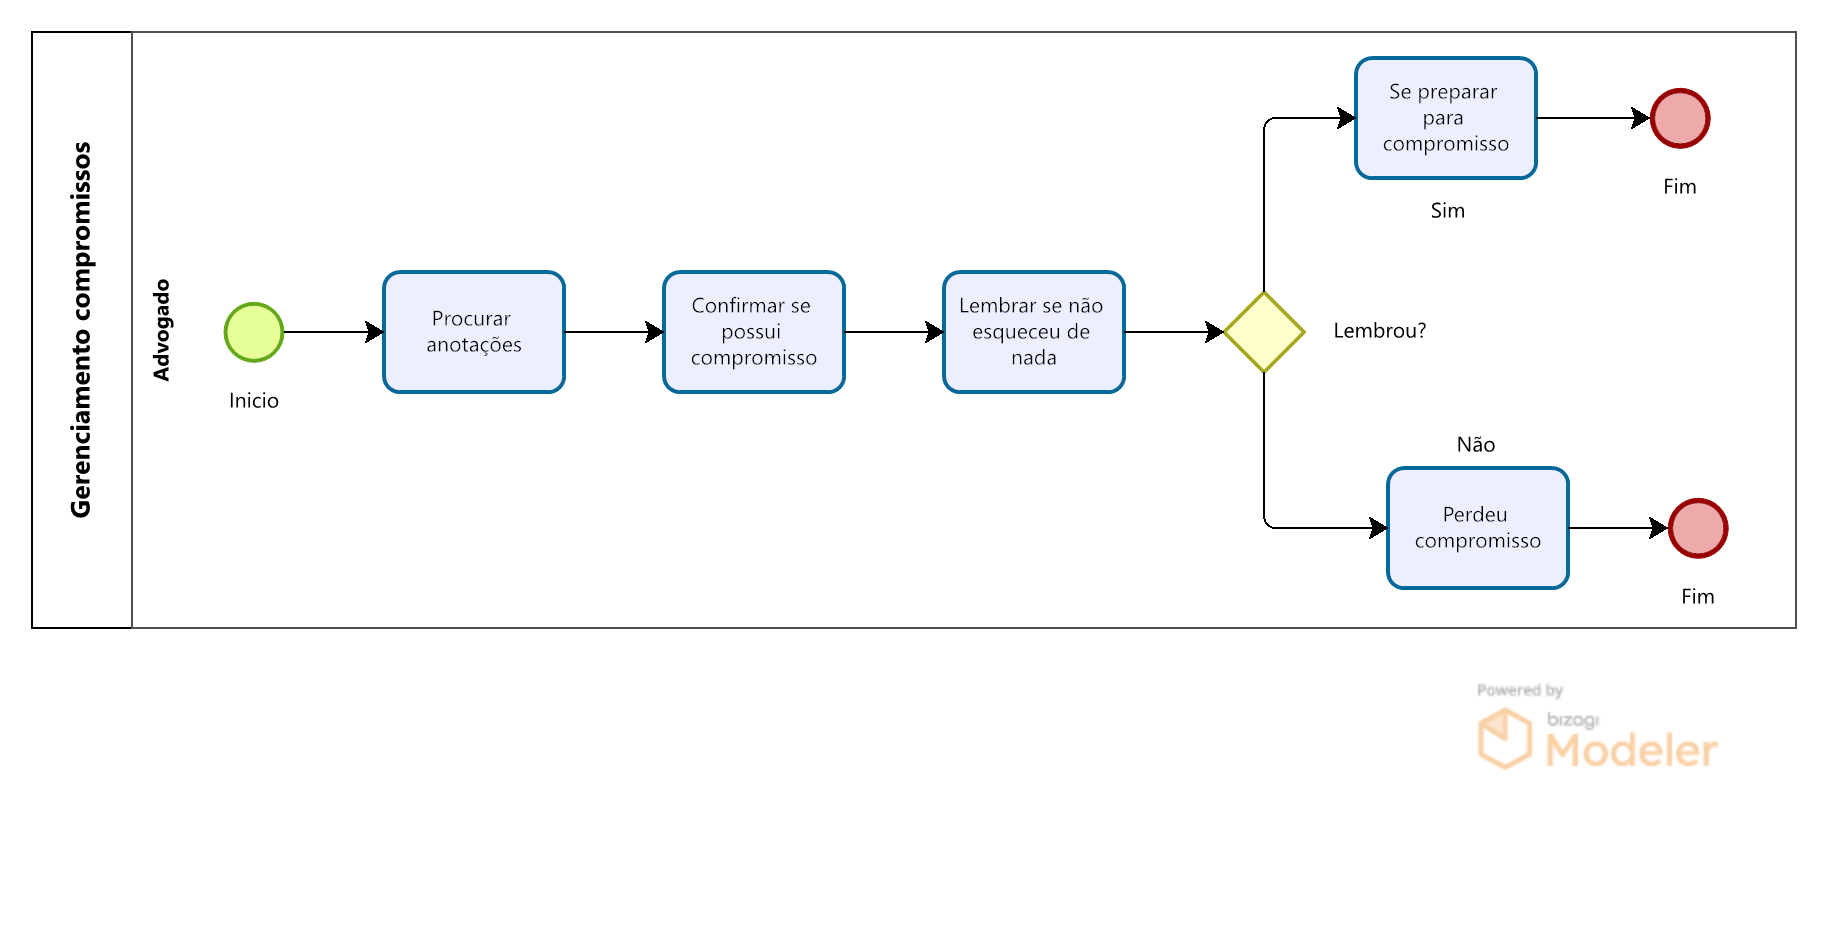
\includegraphics[width=0.8\linewidth]{imagens/BPMN/gerenciarCompromisso.png}
\end{figure}

\begin{figure}
    \centering
    \caption{Processos-(as is)}
    \label{fig:13}
    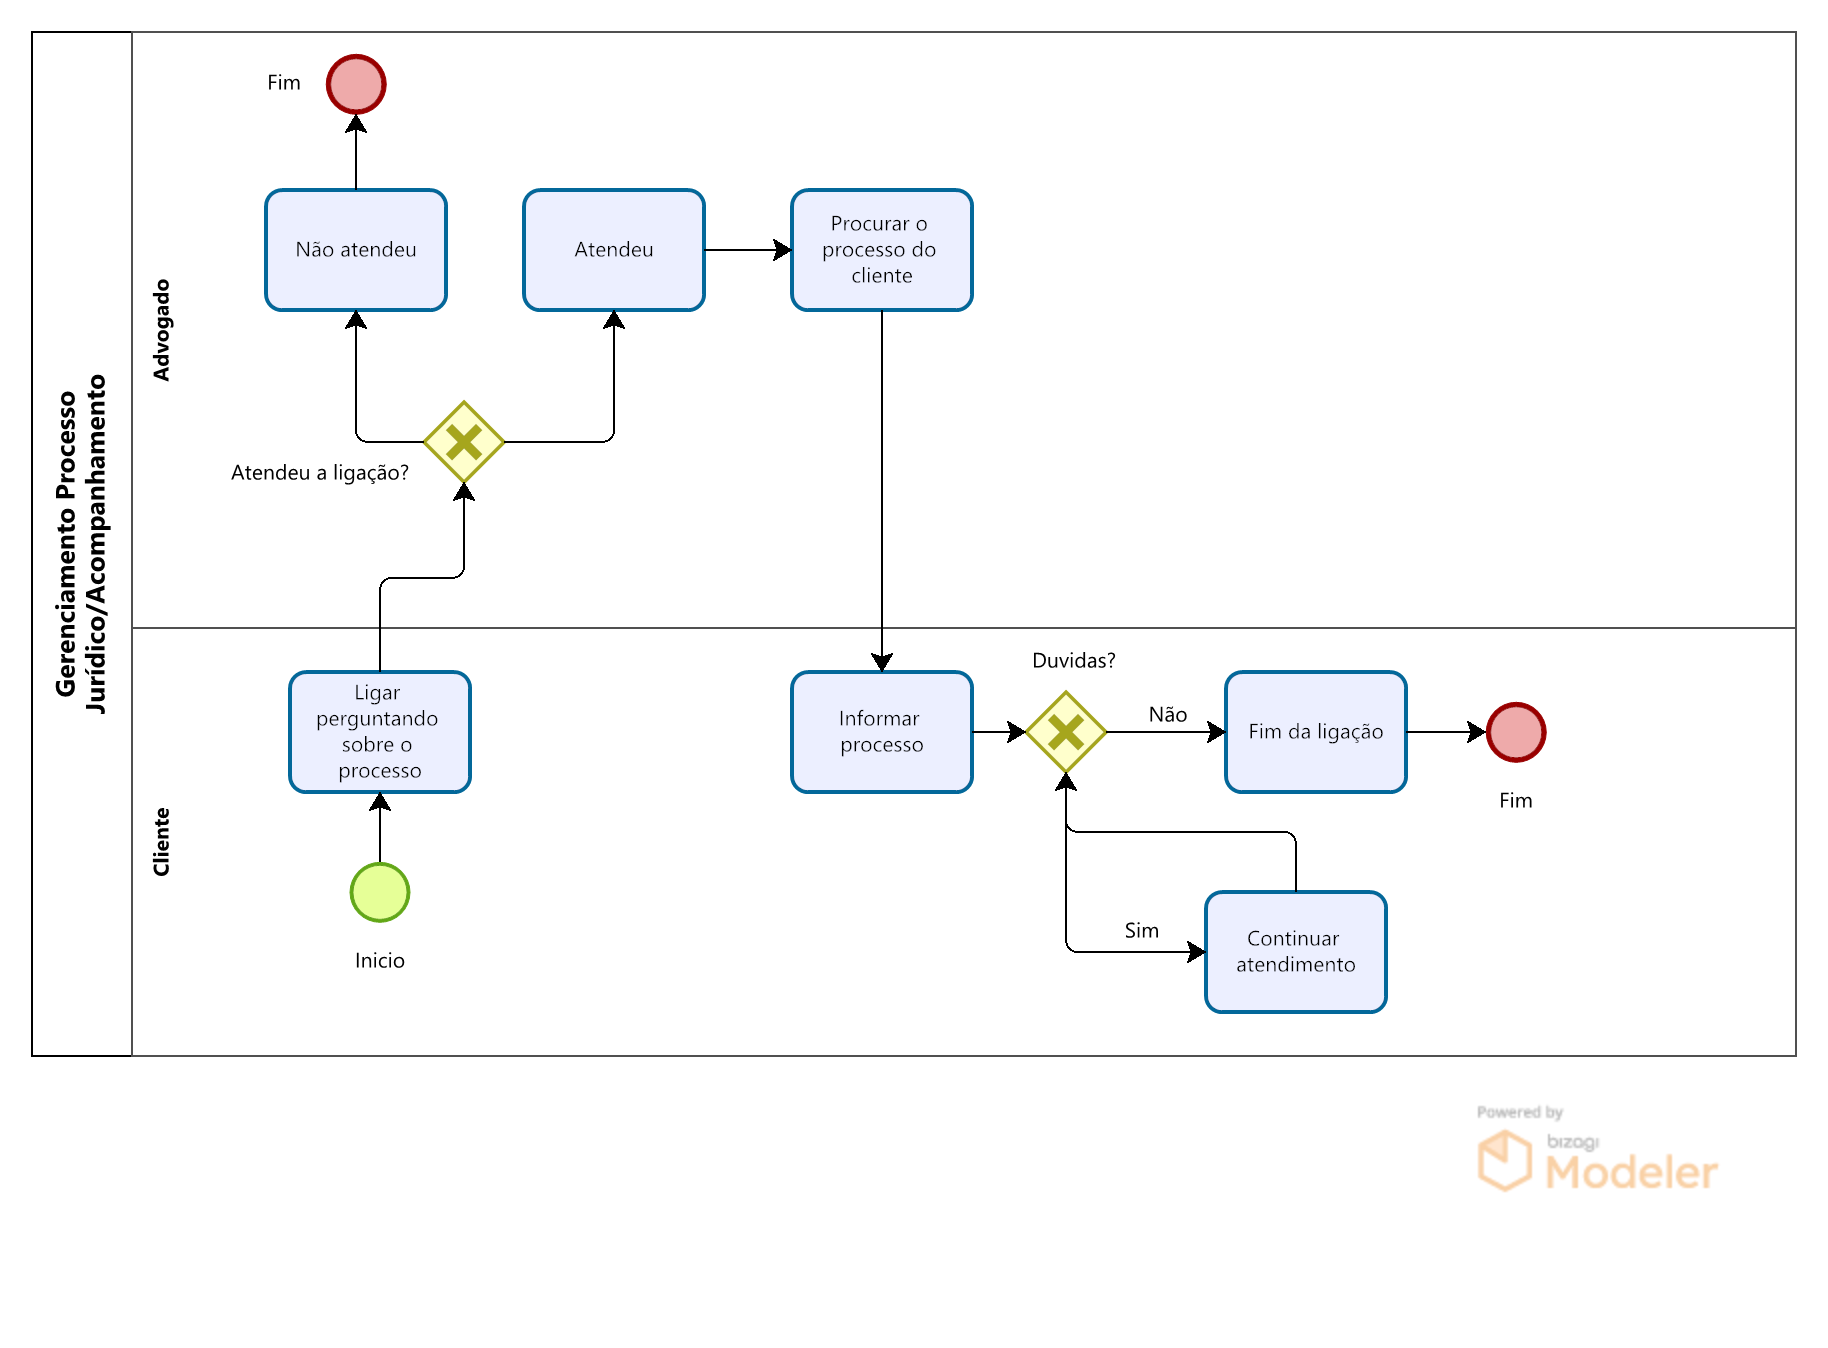
\includegraphics[width=0.8\linewidth]{imagens/BPMN/gerenciarProcesso.png}
\end{figure}

\begin{figure}
    \centering
    \caption{Financeiro-(as is)}
    \label{fig:14}
    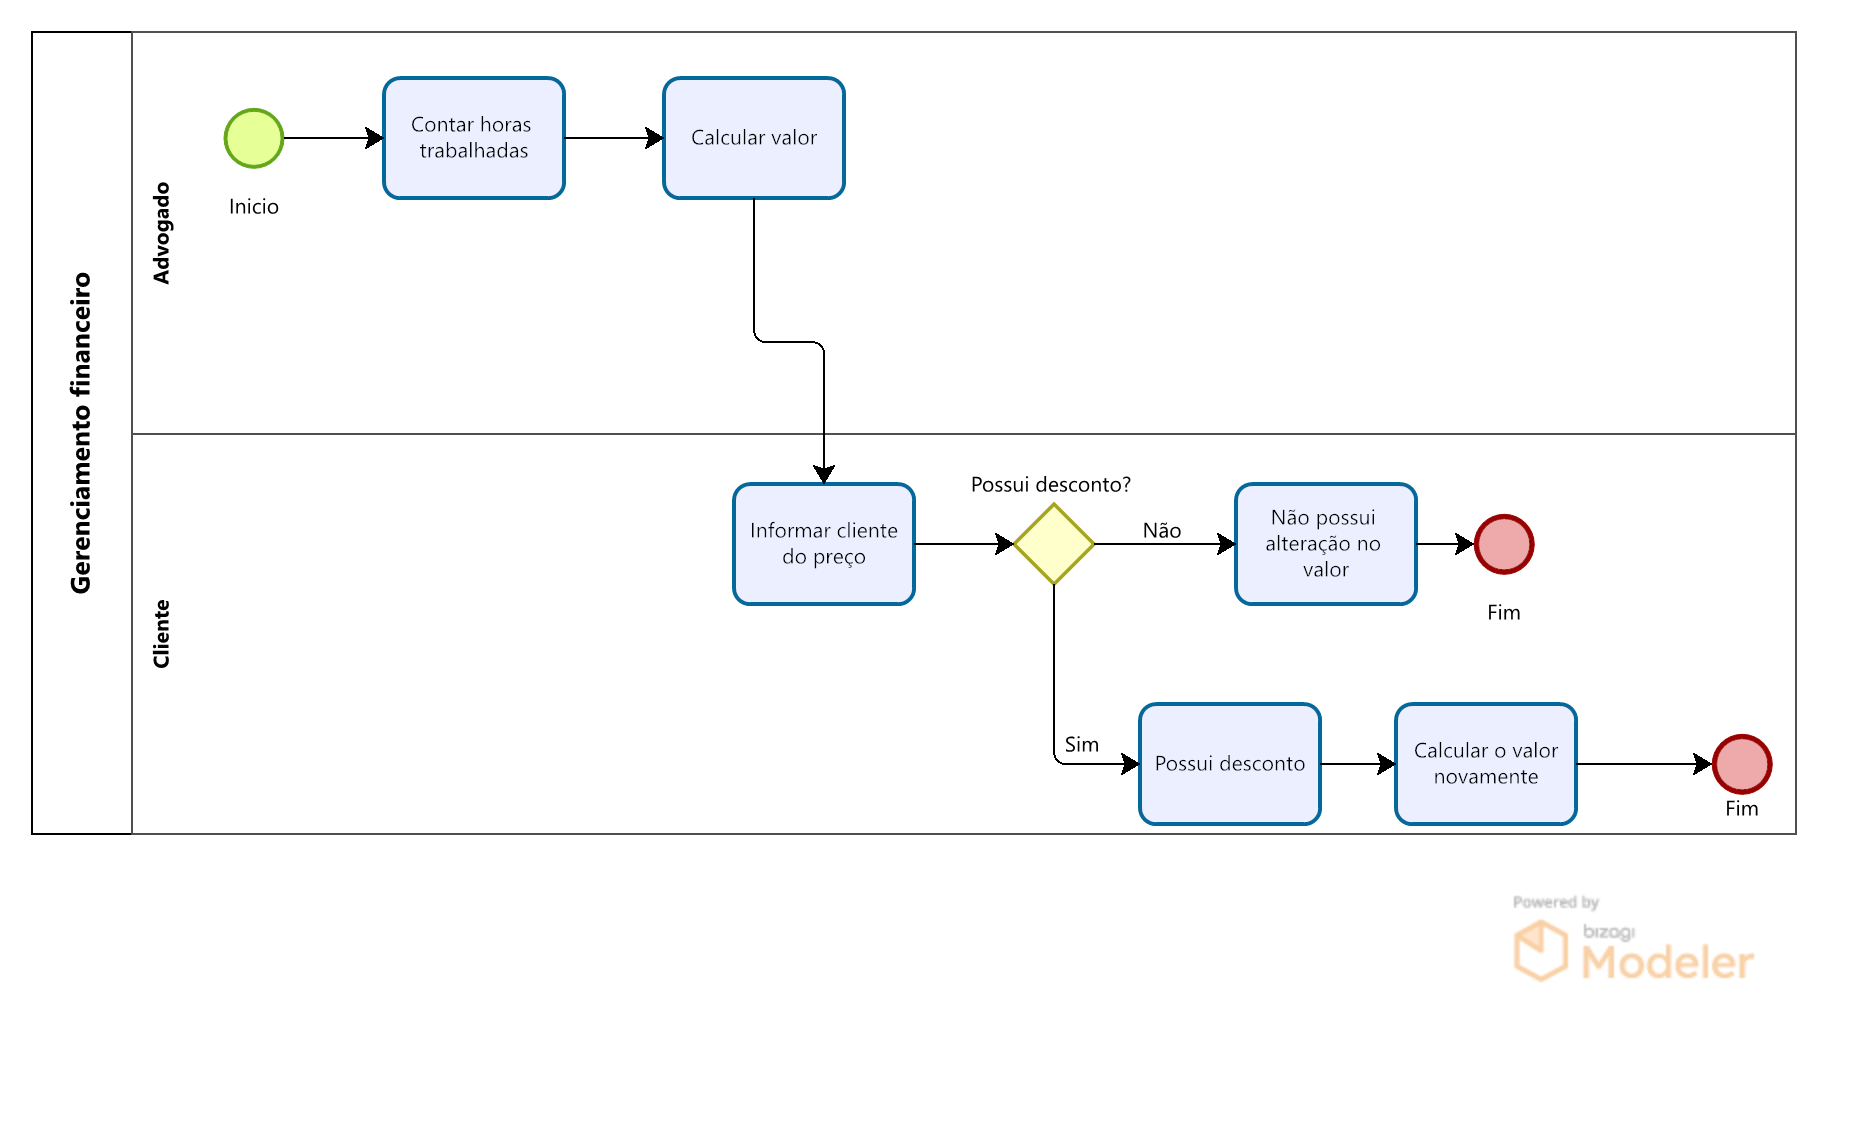
\includegraphics[width=0.8\linewidth]{imagens/BPMN/gerenciarFinanceiro.png}
\end{figure}

\begin{figure}
    \centering
    \caption{Pagamento-(as is)}
    \label{fig:15}
    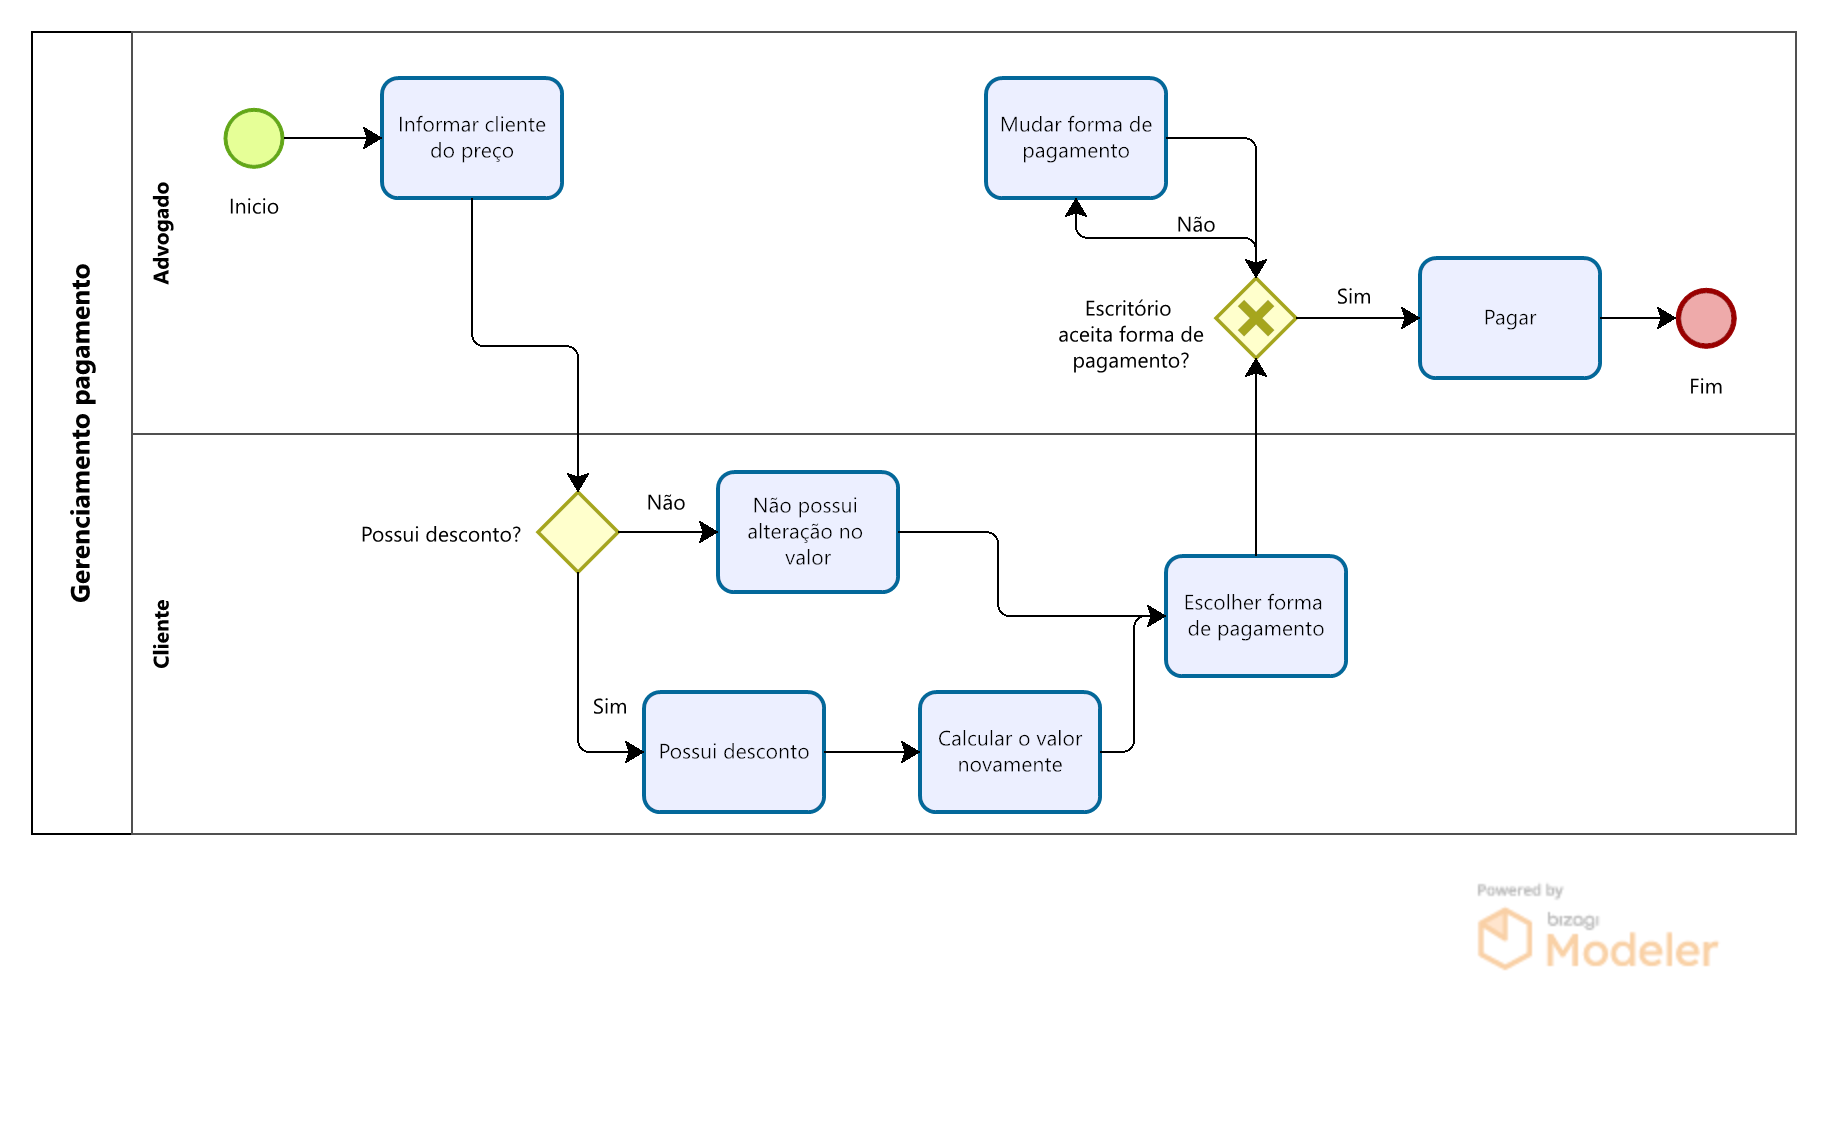
\includegraphics[width=0.8\linewidth]{imagens/BPMN/gerenciarPagamento.png}
\end{figure}

\chapter{Recursos e ambiente de desenovolvimento}\label{sec:4}

"Recursos e ambiente de desenvolvimento" refere-se ao conjunto de ferramentas, tecnologias e recursos disponíveis para os desenvolvedores de software durante o processo de criação de um aplicativo, sistema ou projeto de software.

\cite{miletto2014desenvolvimento}
\section{Linguagem de Programação e Marcação}
PHP para o backend, juntamente com HTML e CSS para o frontend.

\begin{itemize}
    \item \textbf{PHP}: versão 8.2
\end{itemize}

\begin{itemize}
    \item \textbf{HTML}: HTML5
\end{itemize}

\begin{itemize}
    \item \textbf{CSS}: CSS3
\end{itemize}
\cite{converse2003php}
\vspace{\baselineskip}

\section{Frameworks e Bibliotecas}
Utilização do framework Laravel para o backend e Bootstrap para o frontend.

\begin{itemize}
    \item \textbf{Laravel}: versão 8.2
\end{itemize}

\begin{itemize}
    \item \textbf{Bootstrap}: versão 5.0
\end{itemize}

\cite{bento2021desenvolvimento}

\vspace{\baselineskip}

\section{Banco de Dados}
MySQL para armazenar dados relacionados a clientes, processos jurídicos, compromissos e outras informações relevantes.

\cite{milani2007mysql}

\begin{itemize}
    \item \textbf{MySQL}: versão 8.0
\end{itemize}
\vspace{\baselineskip}

\section{Ambiente de Desenvolvimento Integrado (IDE)}
Visual Studio Code para escrever, depurar e testar o código.

\begin{itemize}
    \item \textbf{Visual Studio Code}: versão 1.87.2
\end{itemize}
\vspace{\baselineskip}

\section{Controle de Versão}
Git para gerenciar o código fonte em conjunto com a plataforma GitHub.

\section{Ambiente de Produção}
O ambiente de produção escolhido para hospedar o sistema de advocacia da MR Telles será o InfinityFree, uma plataforma que oferece hospedagem gratuita com suporte a PHP e MySQL. 

\begin{itemize}
    \item \textbf{InfinityFree}: Não possui versão.
\end{itemize}



\cleardoublepage

\postextual

%%Colocar as referências conforme as normas da ABNT, somente as utilizadas no trabalho e presentes neste manuscrito.

%Todas referências deveme star formatadas no formato .bib no arquivo bibliografia.bib para geração automática.

\bibliography{bibliografia}{}

\end{document}